\documentclass[dvipdfmx, 12pt]{article}
\usepackage{mathpazo}
\usepackage{amsmath,amssymb}
\usepackage{array}
\usepackage[hiresbb]{graphicx}
\usepackage{tikz}
\usepackage{textcomp}
\usepackage{dcolumn}
\usepackage{here}
\usepackage{lscape}
\usepackage[top=25truemm,bottom=30truemm,left=25truemm,right=25truemm]{geometry}
\begin{document}

\title{Reference Dependence and Monetary Incentive \\
-Evidence from Major League Baseball-}
\author{Reio Tanji}
\date{}
\maketitle

\leftskip = 25pt
\rightskip = 25pt
  \small
  \textit{
  Many empircal studies have revealed the existance of reference-point dependent preference in field settings, including cases from professional sports players' decision making, whose performance is observed by the manager and is evaluated as their monetary rewards. If there is some incentives, or discontinuous in their rewards that lead the individuals to take behavior that ``appears'' to be driven by the reference dependence, then we should rather think it is caused by the design of the contracts. In this paper, we picked up the case of Major League Baseball players, which Pope and Simonsohn (2011) reported have reference-point dependent preferences about the number of their batting-average. Then, we confirmed the evidences for manipulation in batting-average and other performance indexes, and tested if there exist any monetary incentives that encourage the players to do so. We found three implications: first, there actually exists manipulation in the players' batting-average. Second, surprisingly, there were little evidences that supports the monetary-incentive hypothesis. Third, among the variable indexes, .300 of batting-average was a solid benchmarks for the playrs.
  }

\leftskip = 0pt
\rightskip = 0pt
\normalsize


\section{Introduction}

Reference-point dependence is one of the most important concepts to evaluate outcomes, and it affects agents' following economic behavior. Classical economic models assume that economic agents evaluate their choices/prospects according to the abolute value of (expected) return. On the other hand, Tversky and Kahneman (1992) introduced the behavioral assumption: reference-point dependent preference consider outcomes by the relative value to some target value of the outcomes, reference points. That is, subjects regard the possible outcome as gain or loss from the target. For example, workers feel happy if her/his wage goes up to \$15 per hour, but vice versa if it goes down to \$15, although the absolute value of \$15 is actually the same. In this case, s/he evaluates their new wage with the reference point of the previous one.

In this paper, we deal with the case that outcomes occurs as nonmonetary ones, and then evaluated as monetary rewards: professional sports. In Major League Baseball (MLB), players evalutate the nonmanetary outcomes: indexes that measure the players' performance, with the referene dependent outcomes. We analyzed their contracts with the team they play for, to see if they are designed in order to incentivize the players to take such behavior. As a result, it turned out that there is no monetary incentives there.

Prospect theory consists of two main charactaristics: one is the probability weighting function, and the other is the reference dependence, mentioned above. It enabled us to interpret phenomena that seem inconsistent with the traditional microeconomic theory, and made it possible to understand them with some additional assumptions. Thus, a lot of following researches have been conducted in field and laboratory settings.

Reference dependence is also observed in the behavior of athletes. Pope and Schweizer (2011) found that professional golf players regard ``per,'' the standard number of shots determined according to the difficuly of each hole, as reference points. Also, Allen et al. (2016) argued that marathon runners adjust their finish times before the round number times (just three or four hours), the reference points. Similarly, Pope and Simonsohn (2011) showed the existance of the reference dependence in the MLB, a professional baseball league of America.

MLB position players evaluate themselves by nonmonetary outcomes, the indexes that measure their performance. Moreover, they seems to have some reference points in their self-evaluation, about their batting performance indexes: .300 of batting average. Pope and Simonsohn (2011) have shown that there exists bunching just above .300 of the distribution of this index.

The case of Pope and Simonsohn (2011) differs the former two papers, however, because players receive monetary rewards determined according to their performance.

Suppose the case of the professional golf player. Golf is essentialy competition of the total number of shots they needed to finish the whole tour, regardless of that of each single hole, or whether s/he saves per or not in the hole. Rank of order is determined according to the number of shots, and those with better scores are rewarded. Then, there appears a question that what if there is some monetary incentive to make effort to save per. Or it considers the following situation: when every time s/he saves per in each hole, then s/he can get some additional bonus separated from their total score. In this case, then, making effort to save per can be interpreted as sufficiently ``rational'' choice for the player, although the observed behavior itself appears to be evidence of the reference dependence. In the case of golf, however, there usually does not exist any additional monetary rewards such as ``Save-Per-Bonus.''

On the contrary, in MLB, it is natural to think of such a story. It might not be sufficient to prove that the bunching is caused by reference point dependent utility function about their performance indexes: team managers may assign some monetary incentives for the players to adjust their aspiration level to meet those points, as we described in the example above.

Our most important contribution is this: to conduct analysis that reveals the observed behavior to be in fact reference dependence. First, we confirmed the evidence for the manipulation of the performance indexes around the round numbers, by using McCrary (2008)'s method to test manipulation. We include analysis of not only .300 of batting average, but also other points of batting-average and other indexes, such as homerun or stolen-bases. Second, we made examinations to answer the question, ``Is this observed manipulation truly driven by the reference dependence of the players?'' We applied regression analysis using the data of the players' salary.

Our paper found three important results. First, our examination for manipulation supported the previous study. There observed evidence to show there in fact exists seemingly reference point dependent behavior, where .300 of batting-average works as a reference point. Similar results were obtained about other round numbers of batting-average, and other batting indexes such as on-base percentage or homerun. Second, we found that as a whole, there does not exists any monetary incentive for them: for their fixed part of the salary contract, their monetary rewards are continuous in the each performance index. That is, they behave as they consider these round numbers as reference points, even though they does not receive any additional payment by achieving them. Furthermore, we complement our results, discussing some alternative interpretation about other types of monetary incentives: the part of incentivesed contract, and relation with contract length. And the third, there exists serial changes about the players' index manipulation. .250 of batting-average does not work as a reference point in relatively recent years, while 20 of homerun does only in the recent players. Among them, .300 of batting-average seems to be a solid benchmarks for the players.

This paper proceed as follows. In the Section 2, we review some literature and verify the standpoint of my paper. Section 3 describes the data we availed. Section 4 presents theoretial framework and empirical way to specification, and make some conjecture.  Section 5 show the results of the analysis. Discussion about some alternative interpretation and non-statistical data are included in Section 6. Finally, Section 7 concludes the paper.

\section{Literature Review}

  Tversky and Kahneman (1992) mentioned reference point dependence as one of the two distinct respects of their prospect theory. The most primitive form of reference dependent utility function is:

   \[
  u(x | r) = \begin{cases}
  x - r & \text{ if }x \geq r \\
  \lambda (x - r) & \text{ if }x < r
\end{cases}
  \]
  where $x$ denotes a certain outcome, and $r$ is one of the reference points (Figure \ref{gain-loss}). This agent evaluates the outcome by the difference from the reference point. In adiition, they assume ``loss-aversion'' of the individual, or $\lambda > 1$. Those who have this type of utility function, than they regard same absolute amount of outcome in different way, depending on s/he faces gain or loss situation. ``Diminishing sensitivity,'' which is concave in facing gain and convex in facing loss is an advanced form of this specification (Figure \ref{dim-sen}).

  Diecidue and Van de Ven (2008)`s ``aspiration level'' model added discontinuity assumption: that is, a utility function that ``jumps'' at the reference point (Figure \ref{jump}). When ther exists jump in their utility function, then individuals try to manipulate outcome level, paying addtional cost which was not accepted in the standard continuous utility function. And as a result, there is observed excess mass or bunching around or just above the reference point. As mentioned below, we exploit this assumption to our model in this paper.

  Individuals with such reference-point dependent utility try to adjust their effort level so as to achieve their internal target, or reference point. There is a number of empirical literature that specifies the existence of reference dependence in the field or lab studies. Farber(2008) applied this model to the labor supply of New York cab drivers to show that as soon as they reached daily target sales, they considers to quit, even when they reached it early in each day. Jones(2018) made analysis on the system of American tax payment. He showed that individuals try to manipulate their real payment by substituting it by donation or other charitable action, and that especially when facing losses, they make more effort. This observation is also caused loss-aversion, with the reference point of zero-payment threshold.

  \begin{tabular}{ccc}
    \begin{minipage}[H]{0.3\textwidth}
      \begin{figure}[H]
        \begin{tikzpicture}
          [domain = -2:2, samples = 200, >= stealth]
          \draw[->] (-2,0) -- (2,0) node[right]{$x$};
          \draw[->] (0,-2) -- (0,2) node[above]{$u(x)$};
          \draw plot[domain = 0:1.7] (\x, \x);
          \draw plot[domain = -0.9:0] (\x, {2 * \x});
          \draw (0,0) node [below right] {$r$};
        \end{tikzpicture}
        \scriptsize
        \caption{primitive gain-loss function}
        \label{gain-loss}
      \end{figure}
      \end{minipage} &
      \begin{minipage}[H]{0.3\textwidth}
        \begin{figure}[H]
          \begin{tikzpicture}
            [domain = -2:2, samples = 200, >= stealth]
            \draw[->] (-2,0) -- (2,0) node[right]{$x$};
            \draw[->] (0,-2) -- (0,2) node[above]{$u(x)$};
            \draw plot[domain = 0:1.7] (\x, {sqrt( \x)});
            \draw plot[domain = -1.7:0] (\x, {-sqrt(2 * - \x)});
            \draw (0,0) node [below right] {$r$};
          \end{tikzpicture}
          \scriptsize
          \caption{diminishing sensitivity}
          \label{dim-sen}
        \end{figure}
        \end{minipage}&
        \begin{minipage}[H]{0.3\textwidth}
          \begin{figure}[H]
            \begin{tikzpicture}[domain = 0:4, samples = 200, >= stealth]
              \draw[->](-0.5, 0) -- (4.2, 0) node[right]{$x$};
              \draw[->](0, -0.5) -- (0, 3.7) node[above]{$u(x)$};
              \draw[-](2.2, -0.1) -- (2.2, 0.1);
              \draw[domain=0:2.2,samples=200,>=stealth] plot (\x, {sqrt(\x)});
              \draw[domain=2.2:4.1,samples=200,>=stealth] plot (\x, {sqrt(\x) + 0.8});
              \draw (0, 0) node[below left]{O};
              \draw (2.2, -0.3) node {$r$};
            \end{tikzpicture}
            \scriptsize
            \caption{jump at the reference point}
            \label{jump}
          \end{figure}
        \end{minipage}
      \end{tabular}

\vspace{1zw}


Reference dependence also occurs in the cases of sports. One of the most well-known papers among them is Pope and Schweizer (2011). They obtained the data of professional golf players, to point out that in each hole, players behave as they take ``per'' as the reference point. Specifically, they scceeed their putts, significantly better when the putt was one to save per than when it was one to get ``eagle'' or ``birdie.'' Similarly, Allen \textit{et al} (2016) specified the existance of reference point dependence of marathon runners, using data about the finish time of enormous number of race in the United States. In this case, the distribution of finishing time has excess mass around evry 30 minutes. Note that these cases are common in that the outcomes themselves are nonmonetary ones, and even if they achieve their internal goals, they do not receive any monetary reward for their success. Professional golf players are awarded according to the total number of shots through the whole tour, not to the number of pers they saved.

Pope and Simonsohn (2011) mention a seemingly similar case. They picked up three empirical evidences of round numbers that work as reference points: SAT (a standardized test for college admission in the United States) scores, laboratory experiment, and baseball. In their section of baseball, they picked up the evidence of Major League Baseball (MLB) players. They argue that the players have reference dependent preference in evaluating themselves by a nonmonetary outcome, or their perfonmance index: batting-average (AVG). According to their paper, the position players (batters) pay attention to their batting-average (AVG) especially to finish each season with their batting average of just above .300. They obatined MLB season individual AVG data from 1975 to 2008 and observed position players (= players except for pitchers) with at least 200 at-bats in each season. Then, they found that their distribution of the batting-average has excess mass just above .300, which reveals the existance of manipulation there. Furthermore, they found that players with batting-average of just below .300 are more likely to hit a base-hit and less likely to get a base-on-balls. Both base-hits and base-on-balls avoid the batter from being gotten out, so for the team he belongs to, base-on-balls also have important value to win the game. However, batting-average does not count base-on-balls as the element to raise the number (For the definition of performance indexes, see Appendix), so they prefer getting hit to base-on-balls. Thus, observed behavior they claims is sufficient evidence that shows the existance of round-number reference point dependent preference of the MLB players.

It is true that there is observed behavior similar to the cases of  Allen \textit{et al} (2016): bunching. However, one important thing we have to take care of is that they are professional athlete, and so there exists procedure of contract between the player and the team manager: those who evaluate the player. They propose the players contracts in the next year, after observing the performance they had shown. In other words, the observed excess mass may owe to their monetary value function, not by the preference of themselves. This is the main contribution of my research.

Pope and Simonsohn (2011) stated in their own paper that they conducted analysis only for batting-average, and following research is to be made. So we first search for the round numbers of various batting indexes manipulated by the players. Then, we test if there exists monetary incentive for the players. The team managaers and the players agree the contract that sets fixed additional bonuses, paid when a certain performance index reaching to the point. And then for the players whose indexes are around the cutoff points, making discontinuously large effort, and the following observed bunching can be interpreted as economically rational choice, under the given the contract design. In general, players with their performance index just above these cutoff point and those just below the point have almost same ability as a baseball player. At least, it is natural to think there is no reason to treat players discontinuously better, only because he achieve the cutoff. Then, it is interpreted that it is rather the team manager than the players themselves who have the reference-point dependent preference, which makes the players encouraged to meet their goals. Also if such a type of evaluation is utilized, then the managers can get players that are as skilled as those with .300 of batting average, by relatively reasonable contracts.

On the other hand, if there exists no evidence that team managers evaluate the players by the achievement of the cutoff, then we can say that the observed behavior is truly drawn by their own reference dependence. In addition, the consistency is so strong that even there exists no rational reason, they try to reach there. Analysing this and verify which hypothesis is my main contribution of this paper.

\section{Data Description}

In order to make empirical research, we need information about players' performance, contracts and other details. Then, we obtained panel data that contains these specific information from some open data-source. Each sample is obtained by unit of a single season. Here we explain the specific information about the dataset.

Performance data are obtained obtained from baseball fan website:  \textit{fangraphs} and \textit{Baseball Reference}. We collected information since 1957 season, the year when the qualified number of plate-appearances is regulated. It is the cutoff point to be eligible for the title of leading hitter, the player with the highest batting-average. Stats in each season contains that of only during the regular season, not that of Spring-Training or postseason games. The full-sample is $N=54469$.

Note that we then restrict the sample to the players who appeare to the plate in MLB games enough to be tested, because those with little number of plate-appearances are likely to be evaluated by other elements than their batting skills \ldots skills for pitching or fielding, performance at the minor leagues, or those who injured at the season. Especially about batting-average and on-base percentage, those of players with few plate-appearances are not be regarded as reliable. Pope and Simonsohn (2011) set the cutoff at 200 of at-bats, but alternatively we use 200 plate-appearances as the required number to be considered in our analysis. This is because at-bat does not count the number of base-on-balls or sacrifice bunts, even though they surely appears to the plate and made something to their teams. On the other hand, plate-appearance stands for the number of that their coaches gave him chances of batting. Restricting the sample reduces the number of the sample $N=18143$. The dataset includes the players' plate-appearance, batting-average, on-base percentage, homerun, stolen-base, runs-batted-in, base-hit, all of them are the main indexes of interest in this paper. Also, for the regression analysis, we obtain additional indexes: batting, fielding, and BaseRun, the estimated contribution to the team expressed in the runs they produced, and WPA, or winning percentage added. For further explanations used in our analysis, see Appendix.

Then, here we describe the nature of the indexes. Baseball batting indexes are roughly divided into two types. One is that simply indicates the number of a certain plays, and another is calculated using these numbers, which indicates the rate or the expected number of the plays. Here we call the former ``cumulative index,'' and the latter ``rate index.'' Cumulative index are for example ``base-hit'' or ``homerun,'' or ``stolen-bases.'' Cumulative indexes are irreversible and so they are monotonically increasing in their appearances. That is, so once the players reached a certain number of cumulative indexes such as 20 homeruns, then it does not matter how their performance goes after then. On the other hand, rate indexes can fluctuate: even once they reached their internal goals, it may fall if their performance get worse. Batting-average and on-base percentage are sorted to this type.

Salary data are obtained from \textit{USA TODAY} and \textit{Baseball Prospectus}. We collected annual salary data of the position players who are registered in MLB Roaster at the beginning of each season. It also contains information about other player-specific charactaristics: age, position (such as catcher, 1st-baseman, left-fielder, designated hitter and so on), the teams they signed, and the possession of free agency. We merged this with the play stats in the previous year, because salary is as usually determined based on the performance of the previous season. Because of lack of disclosed information, this dataset contains only that since 1987. Also, because we regard the players' performance is reflected to their annual reward in that of the next year, we cannot merge the stats dataset of 2018. So the latast available season of this is 2017. The aggregated number of the panel is $N=13226$, and the restriction of 200 plate-appearances reduces the number to $N=8915$. Then, here we conduct analysis with two datasets: one that contains salary data (we call this Sample B), while the other does not (Sample A). As we explain in the next section, we use two main analysis: manipulation of performance index (only use play stats) and design of the contracts (needs information about salary). In the former we use Sample A, and in the latter Samlple B. The descriptive statistics of each sample are descripted in Table \ref{sum_A} and Table \ref{sum_B}, respectively.

\begin{table}
  
% Table created by stargazer v.5.2.2 by Marek Hlavac, Harvard University. E-mail: hlavac at fas.harvard.edu
% Date and time: ��, 11 08, 2018 - 14:34:36
% Requires LaTeX packages: dcolumn
\begin{table}[H] \centering
  \caption{Summary Statistics for Sample A}
  \label{sum}
\scriptsize
\begin{tabular}{@{\extracolsep{1.2pt}}lD{.}{.}{-3} D{.}{.}{-3} D{.}{.}{-3} D{.}{.}{-3} D{.}{.}{-3} D{.}{.}{-3} D{.}{.}{-3} }
\\[-1.8ex]\hline
\hline \\[-1.8ex]
Statistic & \multicolumn{1}{c}{N} & \multicolumn{1}{c}{Mean} & \multicolumn{1}{c}{St. Dev.} & \multicolumn{1}{c}{Min} & \multicolumn{1}{c}{Pctl(25)} & \multicolumn{1}{c}{Pctl(75)} & \multicolumn{1}{c}{Max} \\
\hline \\[-1.8ex]
PA & 18,143 & 456.477 & 152.836 & 200 & 320 & 591 & 778 \\
HR & 18,143 & 11.811 & 9.747 & 0 & 4 & 17 & 73 \\
RBI & 18,143 & 51.882 & 26.912 & 4 & 31 & 69 & 165 \\
SB & 18,143 & 7.846 & 10.869 & 0 & 1 & 10 & 130 \\
AVG & 18,143 & .264 & .032 & .135 & .242 & .285 & .394 \\
OBP & 18,143 & .331 & .039 & .174 & .305 & .356 & .609 \\
Age & 18,143 & 28.506 & 4.042 & 18 & 25 & 31 & 46 \\
H & 18,143 & 108.941 & 42.933 & 29 & 72 & 143 & 262 \\
OPS & 18,143 & .738 & .106 & .382 & .665 & .805 & 1.422 \\
\hline \\[-1.8ex]
\end{tabular}
\end{table}

\end{table}

\leftskip = -15pt
\begin{table}
  
% Table created by stargazer v.5.2.2 by Marek Hlavac, Harvard University. E-mail: hlavac at fas.harvard.edu
% Date and time: ��, 11 08, 2018 - 14:49:25
% Requires LaTeX packages: dcolumn
\begin{table}[H] \centering
  \caption{Summary Statistics for Sample B}
  \label{sum_B}
\scriptsize
\begin{tabular}{@{\extracolsep{-5pt}}lD{.}{.}{-3} D{.}{.}{-3} D{.}{.}{-3} D{.}{.}{-3} D{.}{.}{-3} D{.}{.}{-3} D{.}{.}{-3} }
\\[-1.8ex]\hline
\hline \\[-1.8ex]
Statistic & \multicolumn{1}{c}{N} & \multicolumn{1}{c}{Mean} & \multicolumn{1}{c}{St. Dev.} & \multicolumn{1}{c}{Min} & \multicolumn{1}{c}{Pctl(25)} & \multicolumn{1}{c}{Pctl(75)} & \multicolumn{1}{c}{Max} \\
\hline \\[-1.8ex]
Age & 8,915 & 28.714 & 3.901 & 19 & 26 & 31 & 46 \\
PA & 8,915 & 471.946 & 150.890 & 200 & 342 & 605.5 & 778 \\
AVG & 8,915 & .268 & .031 & .146 & .248 & .289 & .394 \\
OBP & 8,915 & .337 & .038 & .174 & .311 & .360 & .609 \\
HR & 8,915 & 13.446 & 10.213 & 0 & 6 & 19 & 73 \\
RBI & 8,915 & 56.339 & 27.621 & 5 & 35 & 74 & 165 \\
SB & 8,915 & 8.534 & 10.851 & 0 & 1 & 11 & 109 \\
H & 8,915 & 114.232 & 42.481 & 30 & 78 & 148 & 262 \\
+WPA & 8,915 & 8.715 & 3.471 & 2.030 & 5.820 & 11.430 & 19.160 \\
-WPA & 8,915 & -8.270 & 2.610 & -15.050 & -10.420 & -6.060 & -2.740 \\
Bat & 8,915 & 3.257 & 16.139 & -44.200 & -7.300 & 11.100 & 116.800 \\
Fld & 8,870 & .304 & 7.482 & -36.100 & -4.000 & 4.400 & 37.000 \\
BsR & 8,915 & .092 & 2.712 & -12.600 & -1.200 & 1.200 & 14.300 \\
Salary & 8,915 & 3,487,838 & 4,487,344 & 62,500 & 512,750 & 4,658,334 & 29,200,000 \\
FA & 8,915 & .168 & .374 & 0 & 0 & 0 & 1 \\
\hline \\[-1.8ex]
\end{tabular}
\end{table}

\end{table}
\leftskip = 0pt

\section{Theoretical Frameworks and Way of Specification}

\subsection{Frameworks}

Baseball is so rich in performance indexes, that records the plays in variable viewpoints. Performance indexes are interpreted as reliable proxies for the skills of the players, so we assume that the players are trying to make them as good as possible. Performance indexes work as clear and valid benchmarks to signal their ability, and team managers evaluate them according to them (also, they include the player-specific charactaristics: age, position and so on). Their evaluation is reflected to monetary rewards to the players, so the players benefit function is described as follows:

\[
F_{it} = F(X_{it}, Z_{it})
\]
where $F$ stands for the monetary reward function to the player $i$ at time $t$, and $X_{it}$ and $Z_{it}$ expresses the value of the index and other player charactaristics, respectively. Players make decision according to this benefit function, and adjust their effort to maximize their utility.

Moreover, each player evaluate himself as an athlete: players directly yield utility by their value of the performance indexes. An alternative explanation is derived by this. That is, players make decision making according to their utility function

\[
U_{it} = U(X_{it})
\]
In this model, players no longer pay attention to their future monetary rewards, and the same in the first model, players decide their effort level to maximize their utility.

Here we assume that before our analysis, we cannot determine which model is proper to interpret the observed behavior of the players: excess mass or bunching around the possible referene points. Our interest is in whether there exists any monetary incentives to lead bunching: Concretely, whether the players' benefit function has discontinuity in a certain performance index. Following Allen \textit{et al} (2016), we first use the assumption of the utility function of Diecidue and Van De Ven (2008)`s ``aspiration level" model. The model presents the form of the utility function with ``notch,''

\[
\lim_{\epsilon \to 0} U_r (r + \epsilon) \neq
\lim_{\epsilon \to 0} U_r (r - \epsilon)
\]
This form of utility function is discontinuous at the reference point $r$.

Also, we consider the possibility that the discontinuous design of the contracts. Similarly to the utility function, notch in the benefit function is expressed as follows:

\[
\lim_{\epsilon \to 0} F_r (r + \epsilon) \neq
\lim_{\epsilon \to 0} F_r (r - \epsilon)
\]

Anyway, the important assumption is that players evaluate their performance index using referene-dependent utility function of themselves or the team manager, and manipulate it in order to maximize their utility. This aspiration results in odd distribution of the index at the end of the season: excess mass around the possible referene point.

In Allen \textit{et al} (2016), they assumed that it is the runners  themselves that have the discontinuous utility function occurs as excess mass around the reference points. On the other hand, we suppose there may be another story. That is, discontinuous utility function of the managers emerges as discontinuous evaluation of the players: salary scheme jumps, depending on whether a ceatain performance index is above or below the reference point. Then, it modifies the income function of the players discontinuous, which results in bunching as the best response of them.

 \subsection{Empirical Method}

  \subsubsection{Test for Bunching}

  First, we test if there is observed any behavior that seems to be related to reference dependent preference. As we explained in the previous sections, manipulation is verified by the observation of bunching, or an excess mass around the possible reference point. To specify the excess mass, we apply the method of regression discontinuity design (RDD).

  RDD is a way to measure the effect of a treatment, such that whether the treatment is assigned or not depends on the threshold of a certain variable (called ``running variable''). Then, comparing the samples just above and just below the threshold is sufficient examination of the treatment, since they are in almost same states except for the existance of the treatment.

  However, there is an important assumption for this specification to be valid (Lee and Lemieux, 2010): continuity of the running variable around the threshold. In other words, individuals must not be able to manipulate the running variable so as to be above the cutpoint. This is because if there exists manipulation, then there occurs selection bias problem, that those who try to be assigned the treatment can adjust their running variable. Therefore, there are some empirical way to test the manipulation of a variable, which is the very method I apply in our analysis. One of the frequently applied methods for this specification is  McCrary(2008)'s local linear density estimation. We avail this to our specification of bunching.

  This test of the manipulation at the cutoff point $c$, proceeds in two steps. First, define $f(.)$ be the density function of the variable $x$ to be tested (here we use the performance indexes). Then we undersmooth the observed density: determine the binsize $b$ of $x$, and obtain the histgram. And finally, we conduct local linear approximation to both just above and below the cutoff point. Note that the optimal bandwidth is to be selected by the fourth order polynominal approximation. Then, we estimate the frequency at the cutoff point, $\Hat{f}(r)$, by fitting the estimated density function from both below and above the cutoff, $\hat{f}^+$ and $\hat{f}^-$, respectively. Finally, we take the difference between $\ln \hat{f}^+$ and $\ln \hat{f}^-$ to calculate the statistics $\theta$. With $\theta$ and its estimator of standard deviation, $t$-tests can be condtructed to specifying manipulation.

  \subsubsection{Monetary Incentive}

  Then, We examine the existance of the monetary incentive. We employ the method of sharp regression discontinuity design (RDD): local linear regression around the possible reference point as the cutoff.
  \[
  w_{it} = \beta_0 X_{it} + \beta_1 \text{ABOVE}_{it}
  \]
  For each player $i$ in the season $t$, $w_{it}$ is loggarithm of their annual salary in next season $t+1$. $X_{it}$ are the value of performance index (batting-average, on-base percentage,\ldots). $\text{ABOVE}_{it}$ is an indicator of the achievement of their goals for the index. That is, if he finished his season with a certain index with above the possible reference point, it takes 1, and otherwise 0, so this is the variable of interest. The bandiwidths in each analysis were selected according to the optimization of Imbens and Kalyanaraman (2009), using polynominal approximation.

  Estimation was conducted in two ways: one only includes the index term and the dummy for achieving their goals in the model, while the other includes term $Z_{it}$, which consists other elements to affect their annual salary. Concretely, it includes player-specific characters (age, team he signed, position,\ldots), and other performance indexes that controls the aspects that covers the players' residual skill, where the performance index $X_{it}$ does not argues. For further explanation, please see Appendix.

  As we mentioned above, usually this method is not applied in this kind of analysis, since RDD can be invalid when individuals can manipulate the running variable, because if they can intentionally control this variable, then anyone who know or want to receive treatment are to manipulate it and so observed sample can be biased. In this research, however, we are interested in the existance itself of the treatment: monetary incentive, so it does not matter if the players did know the (possible) reward or not. Therefore, we regard this way to specification appropreate one to our interests.

  As well as OLS, team, position, or individual fixed effect model estimation was also conducted.


\section{Result}
\subsection{Excess Mass Around The Reference Point}

In this section, we present our main results of analysis. First, we show the results that verifies bunching. Table \ref{Bunch-True} includes the summary of McCrary (2008)'s manipulation tests about the performance indexes that say there is some manipulation occurs. Consistent with Pope and Simonsohn (2011), there actually occurs excess mass around .300, and in addition .250 of batting-average. Also, manipulation were also observed in some of other numbers of other indexes: .350 of on-base percentage, 20 of homeruns, 100 of runs-batted-in, 30 and 40 of stolen-bases, and 200 of base-hits.

\begin{table}
  \small
  \centering
  \begin{tabular}{lcccccc}\hline
    index & type & cutpoint & binsize & bandwidth & $\theta$ & $z$
    \\ \hline \hline
    AVG & rate & .300 & .001 & .019 &  .499 & 7.442*** \\
    & & & & & (.067) & \\
    & & .250 & .001 & .024 & .212 & 5.061*** \\
    & & & & & (.042) & \\
    OBP & rate & .350 & .001 & .024 &  .139 & 2.854** \\
    & & & & & (.049) &  \\
    HR & cumulative & 20 & 1 & 5.309 & .259 & 3.465*** \\
    & & & & & (.075)  & \\
    RBI & cumulative & 100 & 4 & 15.423 & .311 & 3.295*** \\
    & & & & & (.094) & \\
    SB & cumulative & 30 & 1 & 10.000 & .529 & 4.274*** \\
    & & & & & (.124) & \\
    & & 40 & 1 & 11.505 & .481 & 2.764** \\
    & & & & & (.174) & \\
    PA & cumulative & 500 & 1 & .003 & .160 & 2.515* \\
    & & & & &(.063) & \\
    H & cumulative & 200 & 1 & 18.922 & .453 & 2.547 * \\
    & & & & & (.178) & \\ \hline \hline
    Note & \multicolumn{6}{r}{
    ***: $p<0.1\%$, **: $p<1\%$, *: $p<5\%$.
    }\\
    \multicolumn{7}{r}{
    Bandwidth is optimized following the method of McCrary(2008).
    }
  \end{tabular}
  \caption{Test for Manipulation, leastPA $= 200$}
  \label{Bunch-True}
\end{table}

\begin{figure}
  \centering
  \begin{tabular}{ccc}
    \multicolumn{2}{c}{
    \begin{minipage}{.5\textwidth}
      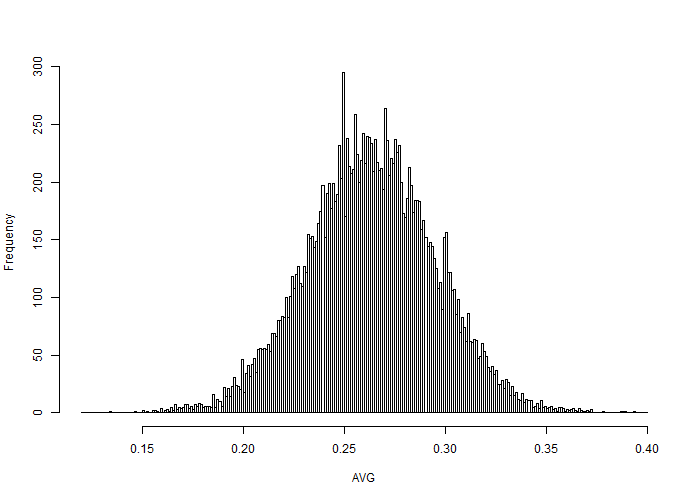
\includegraphics[keepaspectratio, scale = 0.5, angle=0]{graphs/hist_AVG_all.png}
      \caption{Histgram of Batting-Average}
      \label{}
    \end{minipage}
    } \\
    \multicolumn{1}{l}{
    \begin{minipage}{.4\textwidth}
      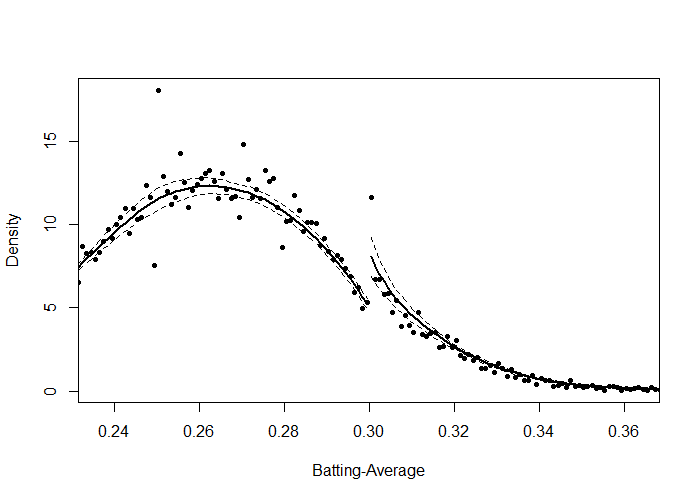
\includegraphics[keepaspectratio, scale = 0.5, angle = 0]{graphs/AVG_300.png}
      \caption{Discontinuity at .300 of AVG}
      \label{DCdensity_AVG_300}
    \end{minipage}
    } & &
    \multicolumn{1}{r}{
    \begin{minipage}{.4\textwidth}
      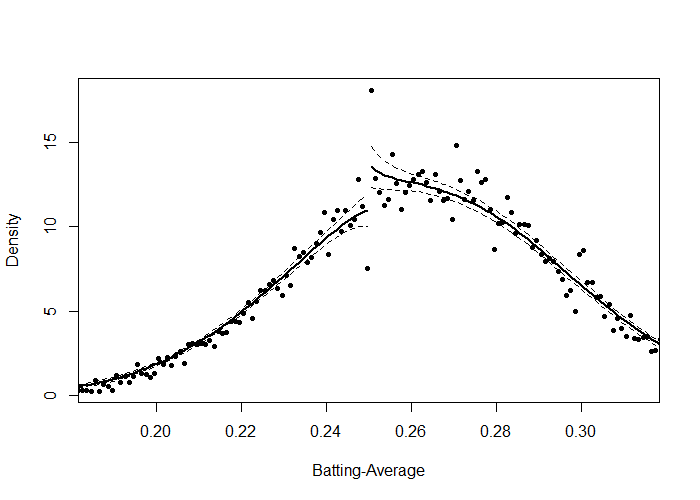
\includegraphics[keepaspectratio, scale = 0.5, angle = 0]{graphs/AVG_250.png}
      \caption{Discontinuity at .250 of AVG}
      \label{DCdensity_AVG_250}
    \end{minipage}
    }
  \end{tabular}
\end{figure}


\begin{figure}
  \centering
  \begin{tabular}{lr}
    \begin{minipage}{.5\textwidth}
      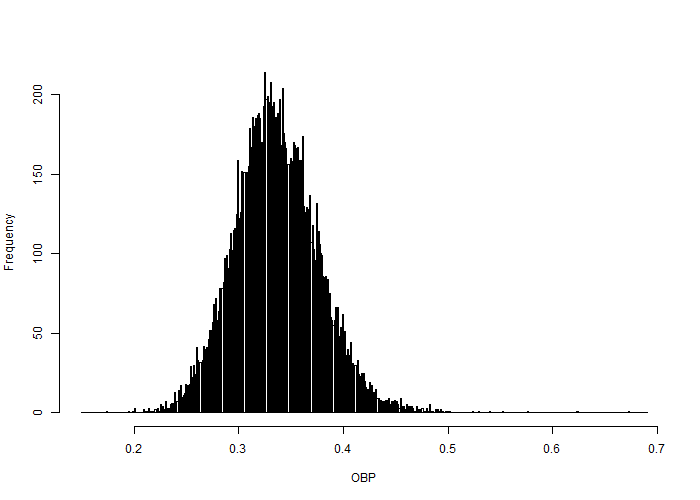
\includegraphics[keepaspectratio, scale = 0.3, angle=0]{graphs/hist_OBP_all.png}
      \caption{Histgram of On-Base Percentage}
      \label{hist_OBP}
    \end{minipage} &

    \begin{minipage}{.5\textwidth}
      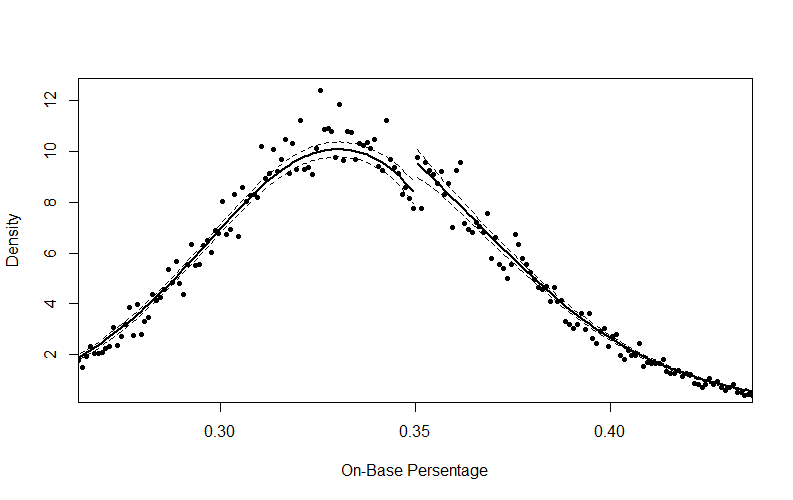
\includegraphics[keepaspectratio, scale = 0.4, angle = 0]{graphs/OBP_350.png}
      \caption{Discontinuity at .350 of OBP}
      \label{DCdensity_OBP_350}

      \end{minipage} \\

      \begin{minipage}{.5\textwidth}
        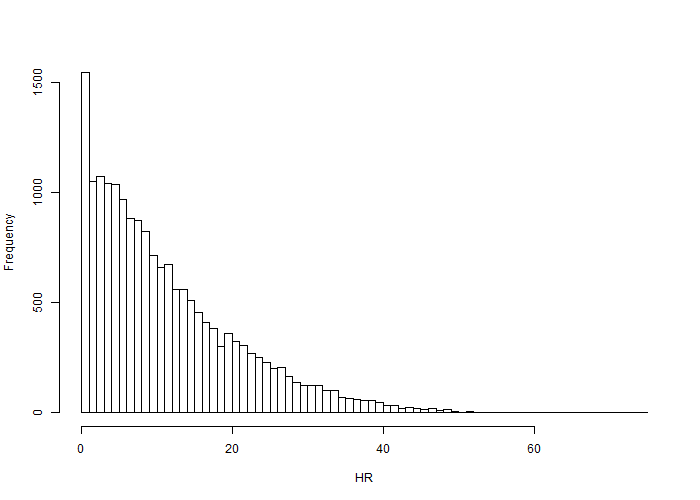
\includegraphics[keepaspectratio, scale = 0.3, angle=0]{graphs/hist_HR_all.png}
        \caption{Histgram of Homerun}
        \label{hist_HR}
        \end{minipage} &

        \begin{minipage}{.5\textwidth}
          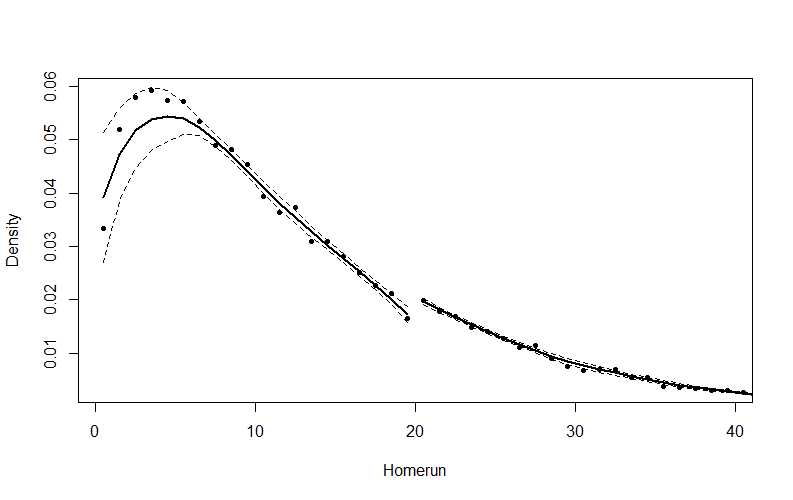
\includegraphics[keepaspectratio, scale = 0.4, angle = 0]{graphs/HR_20.png}
          \caption{Discontinuity at 20 of HR}
          \label{DCdensity_HR}

        \end{minipage}
      \end{tabular}
    \end{figure}

    \begin{figure}
      \centering
      \begin{tabular}{cc}
        \begin{minipage}{.5\textwidth}
          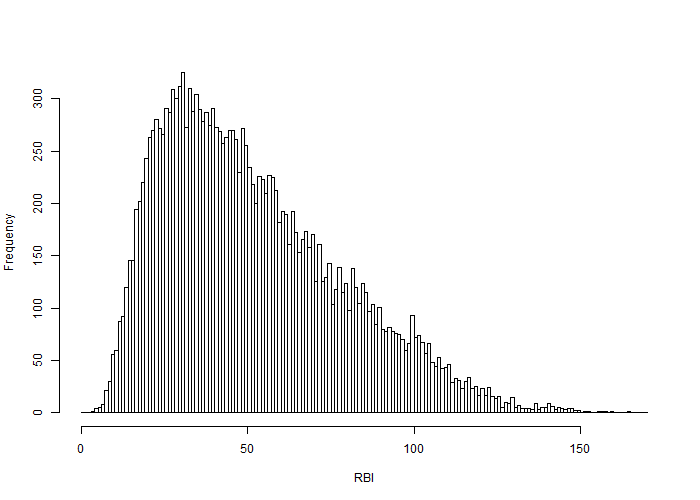
\includegraphics[keepaspectratio, scale = 0.3, angle=0]{graphs/hist_RBI_all.png}
          \caption{Histgram of Runs-Batted-In}
          \label{hist_RBI}
          \end{minipage} &

          \begin{minipage}{.5\textwidth}
            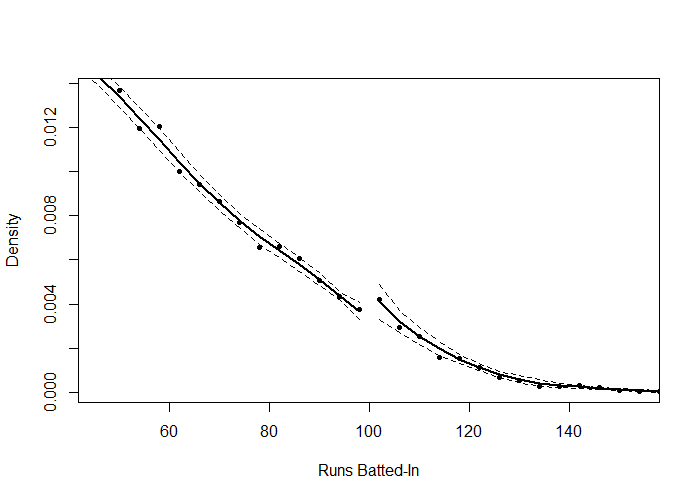
\includegraphics[keepaspectratio, scale = 0.4, angle = 0]{graphs/RBI_100.png}
            \caption{Discontinuity at 100 of RBI}
            \label{DCdensity_RBI_100}

          \end{minipage} \\

          \begin{minipage}{.5\textwidth}
              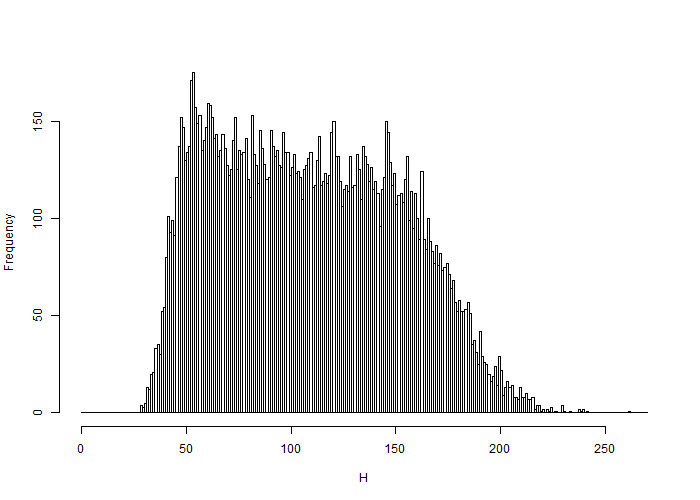
\includegraphics[keepaspectratio, scale = 0.3, angle=0]{graphs/hist_H_all.png}
              \caption{Histgram of Base-Hit}
              \label{hist_H}
          \end{minipage} &

          \begin{minipage}{.5\textwidth}
            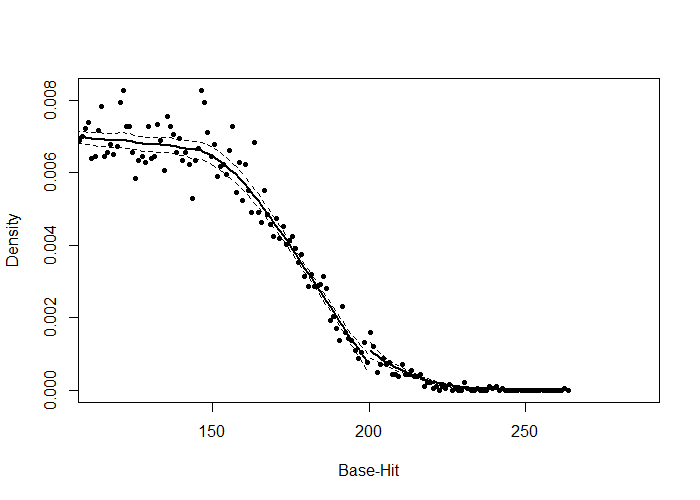
\includegraphics[keepaspectratio, scale = 0.4, angle = 0]{graphs/H_200.png}
            \caption{Discontinuity at 200 of Base-Hit}
            \label{DCdensity_H_200}

          \end{minipage}
        \end{tabular}
      \end{figure}

      \begin{figure}
        \centering
        \begin{tabular}{ccc}
          \multicolumn{2}{c}{
          \begin{minipage}{.5\textwidth}
            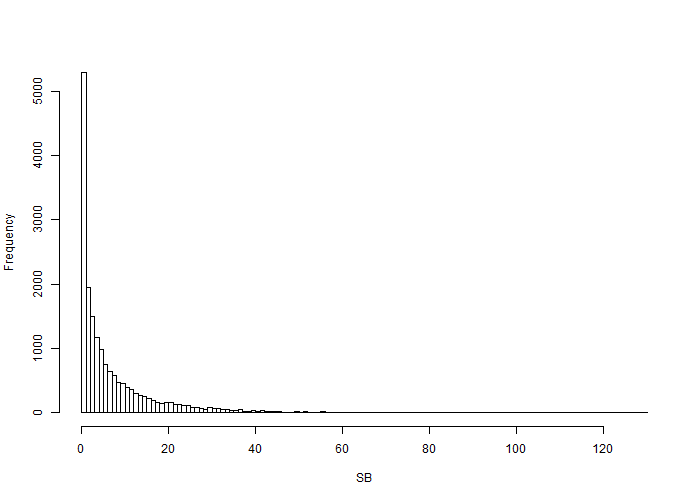
\includegraphics[keepaspectratio, scale = 0.5, angle=0]{graphs/hist_SB_all.png}
            \caption{Histgram of Stolen-Base}
            \label{hist_SB}
          \end{minipage}
          } \\
          \multicolumn{1}{l}{
          \begin{minipage}{.4\textwidth}
            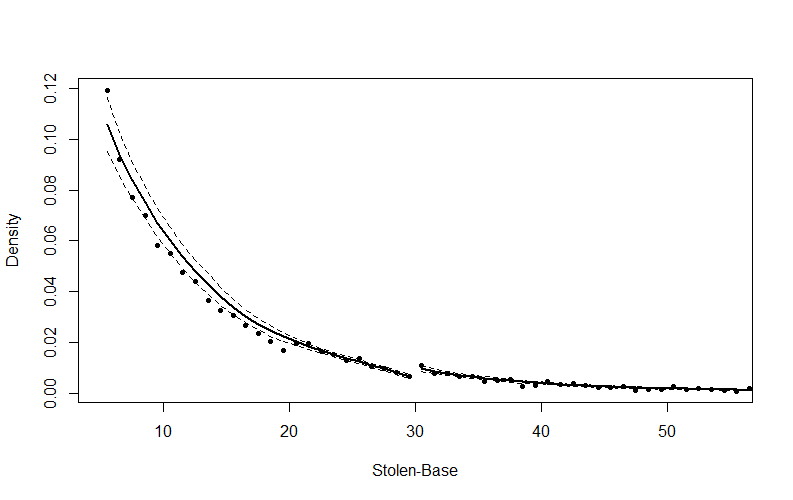
\includegraphics[keepaspectratio, scale = 0.5, angle = 0]{graphs/SB_30.png}
            \caption{Discontinuity at .300 of AVG}
            \label{DCdensity_SB_30}
          \end{minipage}
          } & &
          \multicolumn{1}{r}{
          \begin{minipage}{.4\textwidth}
            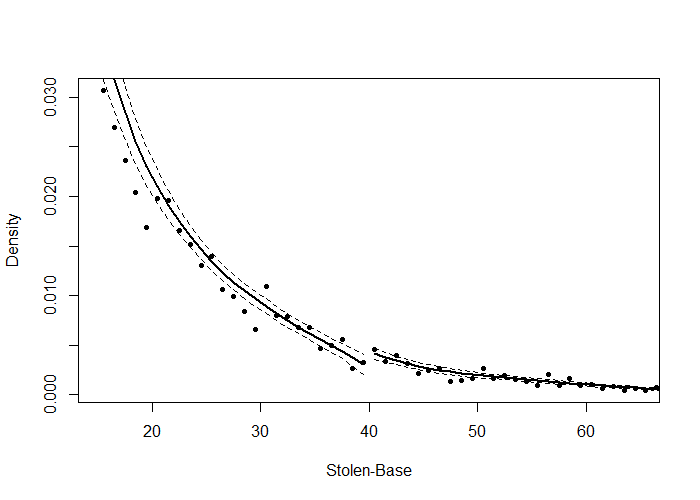
\includegraphics[keepaspectratio, scale = 0.5, angle = 0]{graphs/SB_40.png}
            \caption{Discontinuity at .250 of AVG}
            \label{DCdensity_SB_40}
          \end{minipage}
          }
        \end{tabular}
      \end{figure}

Table \ref{Bunch-True} shows parts of results that denies the existance of excess mass. For precise estimation of bunching, we set the binsizes of undersmoothing artificially: .001 for batting-average and on-base percentage, 1 for homerun (HR), stolen-base (SB), plate-apparance (PA), and base-hit (H), and 4 for runs-batted-in (RBI). Batting-average (AVG) and on-base percentage (OBP) are usually shown by three decimal digits, rounding the fourth decimal digit, so strictly batters with .2995 of batting-average are taken as .300. Homerun, stolen-base, plate-appearance, and base-hit are indexes that takes integer and they earn one for each plate appearances or such a chance to manipulate. Runs-batted-in is also an integer-index, but they can get at most 4 at one plate-appearance, so we set it 4. To confirm the robustness of our results, we repeated this test with various binsize, but we yield essentialy same results. Bandwidths are optimized by calculation, following McCrary (2007).


For batting-average, extending sample size from Pope and Simonsohn (2011) yields similar results: Players manipulate their batting-average. The difference between the estimated frequency according to the approximation below .300 and that of above .300 was significant at .1\% ($z=7.442$) level.

In addition, bunching occurs also in .250 ($z = 5.061$, $p < 0.1\%$). It was not reported in Pope and Simonsohn (2011): for their sample, there was no bunching observed in any other round numbers of batting-average, so it can be related to that the sample size is extended to further old ages. We specifically analyzed this in Section 6.4. Changing binsize to .002 or .005 also yields similar results.

On-base percentage, on the other hand, showed similar tendency in .350, although the significance level was $z=2.854$ (significant at 5\% level). Pope and Simonsohn (2011) reported that they are less likely to get base-on-balls when facing marginal range of batting-average and so they feel of more importance in batting-average than on-base percentage. However, when they face marginal point of on-base percentage, they may try to get more base-on-balls in order to achieve .350.

Bunching also occurs in cumulative indexes. Cumulative ones are irreversible, and so players may feel these indexes are easier to manipulate. As same as batting-average and on-base percentages, however, such manipulation was observed in only limited numbers: not in all the round numbers. For Homerun, bunching occurred only in 20 ($z=3.465, p < 0.1\%$): there may be diminishing sensitivity: 20 is located on above the 75 percentiles of the whole Sample A. Also, stolen-base and base-hit have shown bunching, at 30 ($z=4.274, p < 0.1\%$) and 40 ($z=2.764, p < 1\%$) of stolen-base and 200 in base-hit ($z=2.547, p < 5\%$). Stealing-bases are skill that are talented to limited number of the players, but succeeds with the prpbability of 60\% to alomost 100\%, so those who are evaluated by their number of stolen-bases, it may certain be relatively accessible number to manipulate. 30 and 40 of stolen-bases are also far above the 75 percentiles of all the players.

Base-hit is also manipulated, but the confidence level of the discontinuity was lower than that of batting-average ($z$ = 2.547, $p < 5\%$). Base-hit is a close index to batting-average, for both indexes increase by getting base-hits. It may because the number of base-hit is not regarded as important as batting-average (In most TV live on baseball, they introduce player with his batting-average, not the number of base-hits.) Furtheremore, it can be related that for cumulative indexes, it is not worth ``keeping'' indexes.

And surprisingly such manipulation occurs also in runs-batted-in ($z$=3.295, $p$<0.1\%). Compared to other indexes, runs-batted-in is harder to manipulate, since the number of that depends on the performance of his teammates, and the number they can earn at a single plate-appearance varies from 1 to 4. As in Table \ref{Bunch-True}, the test said that there occurs the evidence in plate-appearances. However, it may insufficient because the optimized bandwidth was smaller than one, even though the number of PAs takes only integers. Setting bandwidth larger than 1, then the result went insignificant.

Summarizing the results, there in fact exists manipulation of the batting indexes and they are possible reference point of the players. However, it occurs in only some parts of round numbers. In the case of marathon runners, Allen et al. (2016), there occured bunching in every round numbers of the goal time, although the size of discontinuity monotonically decreased. That is, it should be considered that the reference points are not determined only because they are round numbers as Pope and Simonsohn (2011) argued. That is, the nature of the reference points are likely to be close to ``per'' in Pope and Schweizer (2011) rather than round numbers; or well, these numbers are monetarily incentivised goals by the team managers. So next, I examine whether there is any monetary bonus in their contract.

\subsection{Existance of Monetary Incentive}

In Section 5.1, we found that there actually exits the player's manipulation for some of the representative indexes. Then in this section, we show whther they are led to aim these goals by their reference dependence, or by their design of the contracts with monetary incentive.

Table \ref{RDD_A} describes the results of RDD analysis on loggarithm of their salary next year, with the cutpoint of each possible reference point. Column ``Other Control'' indicates if the model includes other varivales (other performance indexes, player's age, WPA and dummy for possession of the right of free agency). ``bw type'' indicates the bandwidths used in the model: ``LATE'' includes the sample that are in the optimal bandwidth calculated by Imbens and Kalyyanaraman (), while ``Half-BW'' and ``Double-BW'' are using a half and a twice of the LATE bandwidth, respectively. As a whole, there is no evidence that suports the existance of monetary incenive to make effort for their observed goals. There is no essential difference between the cumulative indexes and rate indexes.

Also, to confirm the robustness of our analysis, we made regression analysis with an interaction term of $X_{it}$ and $\text{ABOVE}_{it}$, which considers the change in average return of the index in argument to their annual salary when the value of the index is above the cutoff point. Each model includes the players that are included in RDD analysis, or those who are located within the optimal bandwidths in RDD. Table \ref{AVG300_A} to \ref{SB40_A} show the results of this analysis for each possible reference points. Consistent with RDD, they give us no evidence of jump of their fixed rewards, except for stolen-bases.



\begin{table}[!]
  \caption{RDD Test for Monetary Incentives}
  \label{RDD_A}
  \tiny
  \centering
  \begin{tabular}{lccccccc}\hline
    index,cutpoint & Other Control & bw type & bandwidth
    & Observations & Estimate & Std. Error & $z$
    \\ \hline \hline
    AVG, .300 & No &LATE & .084 & 8514 & .047 & .061 & .773 \\
    & &Half-BW &  .042 & 5599 & .088 & .075 & 1.174 \\
    & & Double-BW & .170 & 8915  & .067 & .056 & 1.184 \\ \cline{3-8}

    & Yes &LATE & .045 & 5930 & .034 & .056 & .615 \\
    & &Half-BW &  .023 & 3005 & .061 & .077 & .788 \\
    & & Double-BW & .090 & 8605  & .016 & .045 & .354 \\ \hline

    AVG, .250 & No &LATE & .036 & 6110 & .019 & .068 & .286 \\
    & &Half-BW &  .018 & 3496 & .015 & .092 & .161 \\
    & & Double-BW & .072 & 8539  & .034 & .054 & .636 \\ \cline{3-8}

    & Yes &LATE & .048 & 7271 & .070 & .052 & 1.340 \\
    & &Half-BW &  .024 & 4402 & .066 & .069 & .953 \\
    & & Double-BW & .096 & 8810  & .075 & .044 & 1.713 \\ \hline

    HR, 20 & No & LATE & 3.32 & 1315 & .071 & .175 & .406 \\
    & & Half-BW & 1.66 & 562 & .073 & .127 & .576 \\
    & & Double-BW & 6.64 & 2582 & -.004 & .109 & -.034 \\ \cline{3-8}

    & Yes & LATE & 3.30 & 1307 & -.002 & .141 & -.015\\
    & & Half-BW &1.65 & 560 & .030 & .102 & .299 \\
    & & Double-BW & 6.61 & 2558 & -.032 & .088 & -.364 \\ \hline

    OBP, .350 & No &LATE & .044 & 6440 & -.038 & .065 & -.592 \\
    & & Half-BW & .021 & 3542 & -.076 & .089 & -.849 \\
    & & Double-BW & .087 & 8656 & -.029 & .051 & -.570 \\ \cline{3-8}

    & Yes & LATE & .045 & 6525 & -.013 & .049 & -.272 \\
    & & Half-BW & .022 & 3673 & -.055 & .069 & -.807 \\
    & &Double-BW & .089 & 8637 & .004 & .039 & .107 \\ \hline

    RBI, 100 & No & LATE & 4.08 & 393 & .072 & .289 & .250 \\
    & &Half-BW & 2.04 & 228 & .282 & .400 & .707 \\
    & &Double-BW & 8.16 & 714 & .008 & .185 & .043 \\ \cline{3-8}

    & Yes & LATE & 4.04 & 390 & .018 & .209 & .086 \\
    & & Half-BW & 2.02 & 227 & -.042 & .324 & .130 \\
    & & Double-BW & 8.07 & 708 & .056 & .127 & .435 \\ \hline

    H, 200& No & LATE & 3.173 & 75 & -.786 & .396 & -1.985* \\
    & & Half-BW & 1.587 & 35 & .386 & .271 & -1.421 \\
    & & Double-BW & 6.347 & 137 & -.061 & .309 & -.199 \\ \cline{3-8}

    & Yes & LATE & 3.175 & 75 & -.420 & 1.042 & -.403 \\
    & & Half-BW & 1.587 & 35 & -4.779 & .576 & -8.288** \\
    & & Double-BW & 6.349 & 137 & -.109 & .413 & -.265 \\ \hline

    SB, 30 & No & LATE & 3.39 & 282 & .962 & .372 & 2.585** \\
    & &Half-BW & 1.70 & 134 & .920 & .263 & 3.492*** \\
    & &Double-BW & 8.16 & 714 & .008 & .185 & 2.941** \\ \cline{3-8}

    & Yes & LATE & 3.40 & 282 & .379 & .297 & 1.271 \\
    & & Half-BW & 1.70 & 134 & .290 & .249 & 1.163 \\
    & & Double-BW & 6.79 & 533 & .408 & .180 & 2.260* \\ \hline

    SB, 40 & No & LATE & 3.16 & 134 & -1.276 & .453 & -2.818** \\
    & &Half-BW & 1.58 & 56 & -.736 & .383 & -1.924 \\
    & &Double-BW & 6.32 & 245 & -.712 & .313 & -2.274* \\ \cline{3-8}

    & Yes & LATE & 3.16 & 134 & -.346 & .396 & -.875 \\
    & & Half-BW & 1.58 & 56 & -.313 & .429 & -.730 \\
    & & Double-BW & 6.33 & 245 & -.115 & .244 & -.472 \\ \hline

    Note: & \multicolumn{7}{r}{***: $p<0.1\%$, **: $p<1\%$, *: $p<5\%$.} \\
    & \multicolumn{7}{r}{Bandwidth is optimized following the method of Imbens-Kalyanaraman.}
  \end{tabular}
\end{table}

\begin{landscape}
  \begin{table}
    
% Table created by stargazer v.5.2.2 by Marek Hlavac, Harvard University. E-mail: hlavac at fas.harvard.edu
% Date and time: �y, 11 17, 2018 - 21:06:45
\begin{table}[H] \centering 
  \caption{Regression on Log-Salary, Including Interaction Term: around .300} 
  \label{AVG300_A} 
\tiny 
\begin{tabular}{@{\extracolsep{5pt}}lcccccccc} 
\\[-1.8ex]\hline 
\hline \\[-1.8ex] 
 & \multicolumn{8}{c}{\textit{Dependent variable:}} \\ 
\cline{2-9} 
\\[-1.8ex] & \multicolumn{8}{c}{Sal} \\ 
\\[-1.8ex] & \multicolumn{5}{c}{\textit{OLS}} & \multicolumn{3}{c}{\textit{felm}} \\ 
\\[-1.8ex] & (1) & (2) & (3) & (4) & (5) & (6) & (7) & (8)\\ 
\hline \\[-1.8ex] 
 Constant & 11.166$^{***}$ & 9.728$^{***}$ & $-$6.616$^{***}$ & $-$5.049$^{***}$ & $-$5.161$^{***}$ &  &  &  \\ 
  & (.423) & (.399) & (.665) & (.673) & (.669) &  &  &  \\ 
  & & & & & & & & \\ 
 AVG & 11.513$^{***}$ & 11.604$^{***}$ & 11.620$^{***}$ & 4.232$^{***}$ & 4.083$^{***}$ & 4.221$^{***}$ & 3.808$^{**}$ & 3.752$^{**}$ \\ 
  & (1.537) & (1.405) & (1.209) & (1.212) & (1.204) & (1.201) & (1.189) & (1.412) \\ 
  & & & & & & & & \\ 
 AVG\_300 & $-$.169 & $-$.455 & $-$.413 & $-$.261 & $-$.213 & $-$.142 & $-$.069 & $-$.279 \\ 
  & (1.050) & (.954) & (.821) & (.789) & (.784) & (.780) & (.706) & (.918) \\ 
  & & & & & & & & \\ 
 FLD &  & .004 & .006$^{***}$ & .007$^{***}$ & .007$^{***}$ & .007$^{***}$ & .008$^{***}$ & .005$^{**}$ \\ 
  &  & (.002) & (.002) & (.002) & (.002) & (.002) & (.002) & (.002) \\ 
  & & & & & & & & \\ 
 BsR &  & $-$.014$^{**}$ & .009$^{*}$ & .003 & .003 & .003 & .020$^{***}$ & $-$.018$^{**}$ \\ 
  &  & (.005) & (.005) & (.004) & (.004) & (.005) & (.005) & (.005) \\ 
  & & & & & & & & \\ 
 AGE &  &  & 1.005$^{***}$ & .983$^{***}$ & .984$^{***}$ & .997$^{***}$ &  &  \\ 
  &  &  & (.039) & (.037) & (.037) & (.037) &  &  \\ 
  & & & & & & & & \\ 
 AGE\_sq &  &  & $-$.015$^{***}$ & $-$.014$^{***}$ & $-$.014$^{***}$ & $-$.014$^{***}$ &  &  \\ 
  &  &  & (.001) & (.001) & (.001) & (.001) &  &  \\ 
  & & & & & & & & \\ 
 AVG:AVG\_300 & .663 & 1.689 & 1.428 & .930 & .791 & .540 & .160 & 1.077 \\ 
  & (3.429) & (3.118) & (2.681) & (2.577) & (2.560) & (2.549) & (2.312) & (3.000) \\ 
  & & & & & & & & \\ 
\hline \\[-1.8ex] 
WPA &  &  &  & X & X & X & X & X \\ 
FA dummy &  &  &  &  & X & X & X & X \\ 
Season dummies &  & X & X & X & X & X & X & X \\ 
Fixed effects &  &  &  &  &  & Position & Individual & Position \\ 
Observations & 5,960 & 5,930 & 5,930 & 5,930 & 5,930 & 5,930 & 5,930 & 5,930 \\ 
R$^{2}$ & .035 & .215 & .420 & .464 & .471 & .478 & .744 & .276 \\ 
Adjusted R$^{2}$ & .035 & .210 & .416 & .461 & .468 & .473 & .660 & .271 \\ 
Residual Std. Error & 1.286 (df = 5956) & 1.164 (df = 5894) & 1.001 (df = 5892) & .962 (df = 5890) & .956 (df = 5889) & .950 (df = 5880) & .764 (df = 4459) & 1.119 (df = 5882) \\ 
F Statistic & 71.983$^{***}$ (df = 3; 5956) & 46.134$^{***}$ (df = 35; 5894) & 115.152$^{***}$ (df = 37; 5892) & 130.803$^{***}$ (df = 39; 5890) & 131.204$^{***}$ (df = 40; 5889) &  &  &  \\ 
\hline 
\hline \\[-1.8ex] 
\textit{Note:}  & \multicolumn{8}{r}{$^{*}$p$<$0.05; $^{**}$p$<$0.01; $^{***}$p$<$0.001} \\ 
\end{tabular} 
\end{table} 

  \end{table}
\end{landscape}

\begin{landscape}
  \begin{table}
    
% Table created by stargazer v.5.2.2 by Marek Hlavac, Harvard University. E-mail: hlavac at fas.harvard.edu
% Date and time: ��, 11 19, 2018 - 20:00:59
\begin{table}[H] \centering 
  \caption{Regression on Log-Salary, Including Interaction Term: around .250} 
  \label{AVG250_A} 
\tiny 
\begin{tabular}{@{\extracolsep{5pt}}lcccccccc} 
\\[-1.8ex]\hline 
\hline \\[-1.8ex] 
 & \multicolumn{8}{c}{\textit{Dependent variable:}} \\ 
\cline{2-9} 
\\[-1.8ex] & \multicolumn{8}{c}{Sal} \\ 
\\[-1.8ex] & \multicolumn{5}{c}{\textit{OLS}} & \multicolumn{3}{c}{\textit{felm}} \\ 
\\[-1.8ex] & (1) & (2) & (3) & (4) & (5) & (6) & (7) & (8)\\ 
\hline \\[-1.8ex] 
 Constant & 12.039$^{***}$ & 10.292$^{***}$ & $-$6.061$^{***}$ & $-$5.288$^{***}$ & $-$5.513$^{***}$ &  &  &  \\ 
  & (.501) & (.457) & (.632) & (.632) & (.624) &  &  &  \\ 
  & & & & & & & & \\ 
 AVG & 8.003$^{***}$ & 9.795$^{***}$ & 8.623$^{***}$ & 2.156 & 1.906 & 1.554 & 1.960 & 2.722 \\ 
  & (2.145) & (1.926) & (1.636) & (1.621) & (1.599) & (1.592) & (1.557) & (1.909) \\ 
  & & & & & & & & \\ 
 AVG\_250 & $-$.684 & $-$.250 & $-$.597 & $-$.771 & $-$.783 & $-$.923$^{*}$ & $-$.492 & $-$.488 \\ 
  & (.618) & (.555) & (.471) & (.459) & (.452) & (.450) & (.432) & (.539) \\ 
  & & & & & & & & \\ 
 FLD &  & .003 & .004$^{**}$ & .006$^{***}$ & .005$^{***}$ & .006$^{***}$ & .007$^{***}$ & .006$^{***}$ \\ 
  &  & (.002) & (.002) & (.002) & (.001) & (.001) & (.002) & (.002) \\ 
  & & & & & & & & \\ 
 BsR &  & $-$.027$^{***}$ & $-$.001 & $-$.006 & $-$.006 & $-$.006 & .014$^{**}$ & $-$.027$^{***}$ \\ 
  &  & (.005) & (.004) & (.004) & (.004) & (.005) & (.005) & (.005) \\ 
  & & & & & & & & \\ 
 AGE &  &  & 1.021$^{***}$ & 1.013$^{***}$ & 1.019$^{***}$ & 1.030$^{***}$ &  &  \\ 
  &  &  & (.034) & (.033) & (.033) & (.033) &  &  \\ 
  & & & & & & & & \\ 
 AGE\_sq &  &  & $-$.015$^{***}$ & $-$.015$^{***}$ & $-$.015$^{***}$ & $-$.015$^{***}$ &  &  \\ 
  &  &  & (.001) & (.001) & (.001) & (.001) &  &  \\ 
  & & & & & & & & \\ 
 AVG:AVG\_250 & 2.836 & 1.098 & 2.591 & 3.383 & 3.409 & 3.957$^{*}$ & 2.297 & 2.161 \\ 
  & (2.520) & (2.262) & (1.922) & (1.871) & (1.845) & (1.836) & (1.763) & (2.201) \\ 
  & & & & & & & & \\ 
\hline \\[-1.8ex] 
WPA &  &  &  & X & X & X & X & X \\ 
FA dummy &  &  &  &  & X & X & X & X \\ 
Season dummies &  & X & X & X & X & X & X & X \\ 
Fixed effects &  &  &  &  &  & Position & Individual & Position \\ 
Observations & 7,307 & 7,271 & 7,271 & 7,271 & 7,271 & 7,271 & 7,271 & 7,271 \\ 
R$^{2}$ & .032 & .231 & .445 & .476 & .490 & .497 & .735 & .277 \\ 
Adjusted R$^{2}$ & .031 & .227 & .442 & .473 & .487 & .494 & .655 & .273 \\ 
Residual Std. Error & 1.271 (df = 7303) & 1.135 (df = 7235) & .964 (df = 7233) & .937 (df = 7231) & .924 (df = 7230) & .918 (df = 7221) & .758 (df = 5590) & 1.101 (df = 7223) \\ 
F Statistic & 79.391$^{***}$ (df = 3; 7303) & 62.031$^{***}$ (df = 35; 7235) & 156.664$^{***}$ (df = 37; 7233) & 168.232$^{***}$ (df = 39; 7231) & 173.678$^{***}$ (df = 40; 7230) &  &  &  \\ 
\hline 
\hline \\[-1.8ex] 
\textit{Note:}  & \multicolumn{8}{r}{$^{*}$p$<$0.05; $^{**}$p$<$0.01; $^{***}$p$<$0.001} \\ 
\end{tabular} 
\end{table} 

  \end{table}
\end{landscape}

\begin{landscape}
  \begin{table}
    
% Table created by stargazer v.5.2.2 by Marek Hlavac, Harvard University. E-mail: hlavac at fas.harvard.edu
% Date and time: �y, 11 17, 2018 - 21:06:53
\begin{table}[H] \centering 
  \caption{Regression on Log-Salary, Including Interaction Term: around .350} 
  \label{AVG350_A} 
\tiny 
\begin{tabular}{@{\extracolsep{5pt}}lcccccccc} 
\\[-1.8ex]\hline 
\hline \\[-1.8ex] 
 & \multicolumn{8}{c}{\textit{Dependent variable:}} \\ 
\cline{2-9} 
\\[-1.8ex] & \multicolumn{8}{c}{Sal} \\ 
\\[-1.8ex] & \multicolumn{5}{c}{\textit{OLS}} & \multicolumn{3}{c}{\textit{felm}} \\ 
\\[-1.8ex] & (1) & (2) & (3) & (4) & (5) & (6) & (7) & (8)\\ 
\hline \\[-1.8ex] 
 Constant & 10.793$^{***}$ & 9.117$^{***}$ & $-$7.002$^{***}$ & $-$6.993$^{***}$ & $-$7.081$^{***}$ &  &  &  \\ 
  & (.516) & (.472) & (.666) & (.689) & (.683) &  &  &  \\ 
  & & & & & & & & \\ 
 OBP & 10.357$^{***}$ & 11.155$^{***}$ & 10.183$^{***}$ & 5.580$^{***}$ & 5.445$^{***}$ & 5.346$^{***}$ & 6.739$^{***}$ & 7.368$^{***}$ \\ 
  & (1.574) & (1.421) & (1.228) & (1.258) & (1.248) & (1.242) & (1.212) & (1.467) \\ 
  & & & & & & & & \\ 
 OBP\_350 & $-$.132 & $-$.625 & .103 & .080 & .103 & .130 & $-$.832 & $-$.625 \\ 
  & (.888) & (.801) & (.691) & (.676) & (.670) & (.667) & (.620) & (.788) \\ 
  & & & & & & & & \\ 
 FLD &  & .006$^{**}$ & .007$^{***}$ & .008$^{***}$ & .007$^{***}$ & .008$^{***}$ & .007$^{***}$ & .007$^{***}$ \\ 
  &  & (.002) & (.002) & (.002) & (.002) & (.002) & (.002) & (.002) \\ 
  & & & & & & & & \\ 
 BsR &  & $-$.022$^{***}$ & .002 & .001 & .001 & $-$.0003 & .022$^{***}$ & $-$.020$^{***}$ \\ 
  &  & (.005) & (.004) & (.004) & (.004) & (.005) & (.005) & (.005) \\ 
  & & & & & & & & \\ 
 AGE &  &  & 1.016$^{***}$ & 1.021$^{***}$ & 1.021$^{***}$ & 1.037$^{***}$ &  &  \\ 
  &  &  & (.036) & (.035) & (.035) & (.035) &  &  \\ 
  & & & & & & & & \\ 
 AGE\_sq &  &  & $-$.015$^{***}$ & $-$.015$^{***}$ & $-$.015$^{***}$ & $-$.015$^{***}$ &  &  \\ 
  &  &  & (.001) & (.001) & (.001) & (.001) &  &  \\ 
  & & & & & & & & \\ 
 OBP:OBP\_350 & .356 & 1.783 & $-$.237 & $-$.188 & $-$.274 & $-$.321 & 2.166 & 1.790 \\ 
  & (2.516) & (2.269) & (1.960) & (1.915) & (1.898) & (1.889) & (1.760) & (2.232) \\ 
  & & & & & & & & \\ 
\hline \\[-1.8ex] 
WPA &  &  &  & X & X & X & X & X \\ 
FA dummy &  &  &  &  & X & X & X & X \\ 
Season dummies &  & X & X & X & X & X & X & X \\ 
Fixed effects &  &  &  &  &  & Position & Individual & Position \\ 
Observations & 6,656 & 6,620 & 6,620 & 6,620 & 6,620 & 6,620 & 6,620 & 6,620 \\ 
R$^{2}$ & .036 & .231 & .427 & .453 & .462 & .470 & .733 & .260 \\ 
Adjusted R$^{2}$ & .035 & .227 & .424 & .450 & .459 & .466 & .650 & .255 \\ 
Residual Std. Error & 1.267 (df = 6652) & 1.135 (df = 6584) & .980 (df = 6582) & .957 (df = 6580) & .949 (df = 6579) & .943 (df = 6570) & .764 (df = 5042) & 1.114 (df = 6572) \\ 
F Statistic & 81.971$^{***}$ (df = 3; 6652) & 56.520$^{***}$ (df = 35; 6584) & 132.495$^{***}$ (df = 37; 6582) & 139.690$^{***}$ (df = 39; 6580) & 141.515$^{***}$ (df = 40; 6579) &  &  &  \\ 
\hline 
\hline \\[-1.8ex] 
\textit{Note:}  & \multicolumn{8}{r}{$^{*}$p$<$0.05; $^{**}$p$<$0.01; $^{***}$p$<$0.001} \\ 
\end{tabular} 
\end{table} 

  \end{table}
\end{landscape}


\begin{landscape}
  \begin{table}
    
% Table created by stargazer v.5.2.2 by Marek Hlavac, Harvard University. E-mail: hlavac at fas.harvard.edu
% Date and time: �y, 11 17, 2018 - 21:07:04
\begin{table}[H] \centering 
  \caption{Regression on Log-Salary, Including Interaction Term: around 20 HR} 
  \label{HR20_A} 
\tiny 
\begin{tabular}{@{\extracolsep{5pt}}lcccccccc} 
\\[-1.8ex]\hline 
\hline \\[-1.8ex] 
 & \multicolumn{8}{c}{\textit{Dependent variable:}} \\ 
\cline{2-9} 
\\[-1.8ex] & \multicolumn{8}{c}{Sal} \\ 
\\[-1.8ex] & \multicolumn{5}{c}{\textit{OLS}} & \multicolumn{3}{c}{\textit{felm}} \\ 
\\[-1.8ex] & (1) & (2) & (3) & (4) & (5) & (6) & (7) & (8)\\ 
\hline \\[-1.8ex] 
 Constant & 14.429$^{***}$ & 12.592$^{***}$ & $-$6.385$^{***}$ & $-$5.374$^{***}$ & $-$5.750$^{***}$ &  &  &  \\ 
  & (1.092) & (1.045) & (1.381) & (1.425) & (1.409) &  &  &  \\ 
  & & & & & & & & \\ 
 HR & .014 & .036 & .076 & .076 & .074 & .083 & .070 & .036 \\ 
  & (.061) & (.057) & (.046) & (.045) & (.045) & (.045) & (.054) & (.056) \\ 
  & & & & & & & & \\ 
 HR\_20 & $-$1.154 & $-$.474 & .008 & $-$.142 & $-$.051 & $-$.003 & .993 & $-$.847 \\ 
  & (1.393) & (1.313) & (1.055) & (1.035) & (1.022) & (1.025) & (1.248) & (1.295) \\ 
  & & & & & & & & \\ 
 FLD &  & .005 & .010$^{***}$ & .010$^{**}$ & .010$^{***}$ & .010$^{***}$ & .006 & .004 \\ 
  &  & (.004) & (.003) & (.003) & (.003) & (.003) & (.004) & (.004) \\ 
  & & & & & & & & \\ 
 BsR &  & $-$.032$^{**}$ & .001 & $-$.011 & $-$.012 & $-$.022$^{*}$ & $-$.007 & $-$.053$^{***}$ \\ 
  &  & (.011) & (.009) & (.009) & (.009) & (.010) & (.015) & (.012) \\ 
  & & & & & & & & \\ 
 AGE &  &  & 1.109$^{***}$ & 1.107$^{***}$ & 1.123$^{***}$ & 1.127$^{***}$ &  &  \\ 
  &  &  & (.073) & (.072) & (.071) & (.071) &  &  \\ 
  & & & & & & & & \\ 
 AGE\_sq &  &  & $-$.016$^{***}$ & $-$.016$^{***}$ & $-$.016$^{***}$ & $-$.016$^{***}$ &  &  \\ 
  &  &  & (.001) & (.001) & (.001) & (.001) &  &  \\ 
  & & & & & & & & \\ 
 HR:HR\_20 & .061 & .025 & $-$.005 & .0004 & $-$.003 & $-$.007 & $-$.052 & .040 \\ 
  & (.073) & (.069) & (.055) & (.054) & (.054) & (.054) & (.065) & (.068) \\ 
  & & & & & & & & \\ 
\hline \\[-1.8ex] 
WPA &  &  &  & X & X & X & X & X \\ 
FA dummy &  &  &  &  & X & X & X & X \\ 
Season dummies &  & X & X & X & X & X & X & X \\ 
Fixed effects &  &  &  &  &  & Position & Individual & Position \\ 
Observations & 1,315 & 1,307 & 1,307 & 1,307 & 1,307 & 1,307 & 1,307 & 1,307 \\ 
R$^{2}$ & .009 & .172 & .467 & .488 & .501 & .508 & .806 & .212 \\ 
Adjusted R$^{2}$ & .007 & .149 & .452 & .473 & .485 & .489 & .610 & .183 \\ 
Residual Std. Error & 1.203 (df = 1311) & 1.114 (df = 1271) & .894 (df = 1269) & .877 (df = 1267) & .867 (df = 1266) & .864 (df = 1257) & .755 (df = 650) & 1.092 (df = 1259) \\ 
F Statistic & 3.882$^{**}$ (df = 3; 1311) & 7.543$^{***}$ (df = 35; 1271) & 30.087$^{***}$ (df = 37; 1269) & 31.023$^{***}$ (df = 39; 1267) & 31.805$^{***}$ (df = 40; 1266) &  &  &  \\ 
\hline 
\hline \\[-1.8ex] 
\textit{Note:}  & \multicolumn{8}{r}{$^{*}$p$<$0.05; $^{**}$p$<$0.01; $^{***}$p$<$0.001} \\ 
\end{tabular} 
\end{table} 

  \end{table}
\end{landscape}

\begin{landscape}
  \begin{table}
    
% Table created by stargazer v.5.2.2 by Marek Hlavac, Harvard University. E-mail: hlavac at fas.harvard.edu
% Date and time: �y, 11 17, 2018 - 21:25:13
\begin{table}[H] \centering 
  \caption{Regression on Log-Salary, Including Interaction Term: around 30 SB} 
  \label{SB30_A} 
\tiny 
\begin{tabular}{@{\extracolsep{5pt}}lcccccccc} 
\\[-1.8ex]\hline 
\hline \\[-1.8ex] 
 & \multicolumn{8}{c}{\textit{Dependent variable:}} \\ 
\cline{2-9} 
\\[-1.8ex] & \multicolumn{8}{c}{Sal} \\ 
\\[-1.8ex] & \multicolumn{5}{c}{\textit{OLS}} & \multicolumn{3}{c}{\textit{felm}} \\ 
\\[-1.8ex] & (1) & (2) & (3) & (4) & (5) & (6) & (7) & (8)\\ 
\hline \\[-1.8ex] 
 Constant & 13.466$^{***}$ & 8.006$^{*}$ & $-$4.126 & $-$3.729 & $-$2.949 &  &  &  \\ 
  & (3.672) & (3.191) & (3.586) & (3.651) & (3.675) &  &  &  \\ 
  & & & & & & & & \\ 
 SB & .029 & .167 & $-$.036 & $-$.041 & $-$.052 & $-$.067 & .075 & .145 \\ 
  & (.132) & (.114) & (.099) & (.099) & (.099) & (.096) & (.185) & (.113) \\ 
  & & & & & & & & \\ 
 SB\_30 & 12.468$^{**}$ & 13.567$^{***}$ & 2.544 & 2.234 & 1.579 & .816 & 7.200 & 12.144$^{**}$ \\ 
  & (4.569) & (3.972) & (3.531) & (3.526) & (3.541) & (3.464) & (6.586) & (3.947) \\ 
  & & & & & & & & \\ 
 FLD &  & .003 & .007 & .007 & .007 & .008 & .013 & .005 \\ 
  &  & (.007) & (.006) & (.006) & (.005) & (.005) & (.011) & (.006) \\ 
  & & & & & & & & \\ 
 BAT &  & .028$^{***}$ & .023$^{***}$ & .015$^{**}$ & .014$^{*}$ & .017$^{**}$ & .019 & .021$^{**}$ \\ 
  &  & (.003) & (.003) & (.006) & (.006) & (.006) & (.010) & (.007) \\ 
  & & & & & & & & \\ 
 AGE &  &  & 1.142$^{***}$ & 1.150$^{***}$ & 1.105$^{***}$ & 1.132$^{***}$ &  &  \\ 
  &  &  & (.174) & (.174) & (.176) & (.172) &  &  \\ 
  & & & & & & & & \\ 
 AGE\_sq &  &  & $-$.018$^{***}$ & $-$.018$^{***}$ & $-$.017$^{***}$ & $-$.017$^{***}$ &  &  \\ 
  &  &  & (.003) & (.003) & (.003) & (.003) &  &  \\ 
  & & & & & & & & \\ 
 SB:SB\_30 & $-$.391$^{*}$ & $-$.444$^{**}$ & $-$.071 & $-$.061 & $-$.039 & $-$.013 & $-$.230 & $-$.397$^{**}$ \\ 
  & (.158) & (.137) & (.122) & (.122) & (.122) & (.119) & (.229) & (.136) \\ 
  & & & & & & & & \\ 
\hline \\[-1.8ex] 
WPA &  &  &  & X & X & X & X & X \\ 
FA dummy &  &  &  &  & X & X & X & X \\ 
Season dummies &  & X & X & X & X & X & X & X \\ 
Fixed effects &  &  &  &  &  & Position & Individual & Position \\ 
Observations & 282 & 282 & 282 & 282 & 282 & 282 & 282 & 282 \\ 
R$^{2}$ & .075 & .472 & .628 & .633 & .636 & .675 & .915 & .523 \\ 
Adjusted R$^{2}$ & .065 & .397 & .571 & .573 & .576 & .608 & .651 & .430 \\ 
Residual Std. Error & 1.229 (df = 278) & .988 (df = 246) & .833 (df = 244) & .830 (df = 242) & .828 (df = 241) & .796 (df = 233) & .751 (df = 68) & .960 (df = 235) \\ 
F Statistic & 7.559$^{***}$ (df = 3; 278) & 6.276$^{***}$ (df = 35; 246) & 11.110$^{***}$ (df = 37; 244) & 10.684$^{***}$ (df = 39; 242) & 10.537$^{***}$ (df = 40; 241) &  &  &  \\ 
\hline 
\hline \\[-1.8ex] 
\textit{Note:}  & \multicolumn{8}{r}{$^{*}$p$<$0.05; $^{**}$p$<$0.01; $^{***}$p$<$0.001} \\ 
\end{tabular} 
\end{table} 

  \end{table}
\end{landscape}

\begin{landscape}
  \begin{table}
    
% Table created by stargazer v.5.2.2 by Marek Hlavac, Harvard University. E-mail: hlavac at fas.harvard.edu
% Date and time: �y, 11 17, 2018 - 21:07:14
\begin{table}[H] \centering 
  \caption{Regression on Log-Salary, Including Interaction Term: around 40 SB} 
  \label{SB40_A} 
\tiny 
\begin{tabular}{@{\extracolsep{5pt}}lcccccccc} 
\\[-1.8ex]\hline 
\hline \\[-1.8ex] 
 & \multicolumn{8}{c}{\textit{Dependent variable:}} \\ 
\cline{2-9} 
\\[-1.8ex] & \multicolumn{8}{c}{Sal} \\ 
\\[-1.8ex] & \multicolumn{5}{c}{\textit{OLS}} & \multicolumn{3}{c}{\textit{felm}} \\ 
\\[-1.8ex] & (1) & (2) & (3) & (4) & (5) & (6) & (7) & (8)\\ 
\hline \\[-1.8ex] 
 Constant & .097 & 2.795 & $-$6.186 & $-$5.258 & $-$3.914 &  &  &  \\ 
  & (6.865) & (6.575) & (6.345) & (6.781) & (6.974) &  &  &  \\ 
  & & & & & & & & \\ 
 SB & .392$^{*}$ & .287 & .191 & .183 & .148 & .148 & .679$^{*}$ & .187 \\ 
  & (.182) & (.174) & (.155) & (.158) & (.163) & (.163) & (.265) & (.182) \\ 
  & & & & & & & & \\ 
 SB\_40 & 20.483$^{*}$ & 7.339 & 5.634 & 5.543 & 5.082 & 7.669 & 37.152$^{**}$ & 7.632 \\ 
  & (8.497) & (8.171) & (7.281) & (7.430) & (7.461) & (7.511) & (12.783) & (8.367) \\ 
  & & & & & & & & \\ 
 FLD &  & .003 & .005 & .005 & .005 & .008 & .021 & .005 \\ 
  &  & (.009) & (.008) & (.008) & (.008) & (.009) & (.020) & (.009) \\ 
  & & & & & & & & \\ 
 BAT &  & .025$^{***}$ & .023$^{***}$ & .020$^{*}$ & .020$^{*}$ & .021$^{*}$ & $-$.001 & .017 \\ 
  &  & (.005) & (.004) & (.009) & (.009) & (.009) & (.020) & (.010) \\ 
  & & & & & & & & \\ 
 AGE &  &  & .763$^{**}$ & .751$^{**}$ & .751$^{**}$ & .745$^{**}$ &  &  \\ 
  &  &  & (.239) & (.242) & (.243) & (.245) &  &  \\ 
  & & & & & & & & \\ 
 AGE\_sq &  &  & $-$.011$^{**}$ & $-$.011$^{**}$ & $-$.011$^{**}$ & $-$.011$^{*}$ &  &  \\ 
  &  &  & (.004) & (.004) & (.004) & (.004) &  &  \\ 
  & & & & & & & & \\ 
 SB:SB\_40 & $-$.537$^{*}$ & $-$.205 & $-$.152 & $-$.149 & $-$.134 & $-$.198 & $-$.956$^{**}$ & $-$.203 \\ 
  & (.218) & (.210) & (.187) & (.191) & (.192) & (.194) & (.328) & (.215) \\ 
  & & & & & & & & \\ 
\hline \\[-1.8ex] 
WPA &  &  &  & X & X & X & X & X \\ 
FA dummy &  &  &  &  & X & X & X & X \\ 
Season dummies &  & X & X & X & X & X & X & X \\ 
Fixed effects &  &  &  &  &  & Position & Individual & Position \\ 
Observations & 134 & 134 & 134 & 134 & 134 & 134 & 134 & 134 \\ 
R$^{2}$ & .062 & .519 & .634 & .636 & .638 & .665 & .949 & .559 \\ 
Adjusted R$^{2}$ & .041 & .353 & .499 & .490 & .488 & .494 & .645 & .348 \\ 
Residual Std. Error & 1.158 (df = 130) & .951 (df = 99) & .837 (df = 97) & .845 (df = 95) & .846 (df = 94) & .841 (df = 88) & .705 (df = 19) & .955 (df = 90) \\ 
F Statistic & 2.875$^{*}$ (df = 3; 130) & 3.137$^{***}$ (df = 34; 99) & 4.674$^{***}$ (df = 36; 97) & 4.363$^{***}$ (df = 38; 95) & 4.257$^{***}$ (df = 39; 94) &  &  &  \\ 
\hline 
\hline \\[-1.8ex] 
\textit{Note:}  & \multicolumn{8}{r}{$^{*}$p$<$0.05; $^{**}$p$<$0.01; $^{***}$p$<$0.001} \\ 
\end{tabular} 
\end{table} 

  \end{table}
\end{landscape}

\begin{landscape}
  \begin{table}
    
% Table created by stargazer v.5.2.2 by Marek Hlavac, Harvard University. E-mail: hlavac at fas.harvard.edu
% Date and time: �y, 11 17, 2018 - 21:07:29
\begin{table}[H] \centering 
  \caption{Regression on Log-Salary, Including Interaction Term: around 100 RBI} 
  \label{RBI100_A} 
\tiny 
\begin{tabular}{@{\extracolsep{5pt}}lcccccccc} 
\\[-1.8ex]\hline 
\hline \\[-1.8ex] 
 & \multicolumn{8}{c}{\textit{Dependent variable:}} \\ 
\cline{2-9} 
\\[-1.8ex] & \multicolumn{8}{c}{Sal} \\ 
\\[-1.8ex] & \multicolumn{5}{c}{\textit{OLS}} & \multicolumn{3}{c}{\textit{felm}} \\ 
\\[-1.8ex] & (1) & (2) & (3) & (4) & (5) & (6) & (7) & (8)\\ 
\hline \\[-1.8ex] 
 Constant & 17.552$^{*}$ & 13.364$^{*}$ & $-$3.577 & $-$3.767 & $-$3.797 &  &  &  \\ 
  & (7.013) & (6.189) & (5.256) & (5.174) & (5.183) &  &  &  \\ 
  & & & & & & & & \\ 
 RBI & $-$.023 & .001 & $-$.017 & $-$.007 & $-$.007 & $-$.011 & .049 & .007 \\ 
  & (.072) & (.063) & (.052) & (.051) & (.051) & (.050) & (.078) & (.061) \\ 
  & & & & & & & & \\ 
 RBI\_100 & $-$11.458 & $-$3.512 & $-$2.428 & $-$1.810 & $-$1.692 & $-$2.447 & .582 & $-$4.377 \\ 
  & (8.459) & (7.492) & (6.115) & (5.971) & (6.001) & (5.966) & (8.865) & (7.250) \\ 
  & & & & & & & & \\ 
 FLD &  & $-$.0002 & .004 & .004 & .004 & .007 & $-$.004 & .003 \\ 
  &  & (.005) & (.004) & (.004) & (.004) & (.004) & (.007) & (.005) \\ 
  & & & & & & & & \\ 
 BsR &  & $-$.035$^{*}$ & .001 & $-$.008 & $-$.008 & $-$.016 & .034 & $-$.046$^{**}$ \\ 
  &  & (.014) & (.012) & (.012) & (.012) & (.013) & (.023) & (.015) \\ 
  & & & & & & & & \\ 
 AGE &  &  & 1.185$^{***}$ & 1.195$^{***}$ & 1.195$^{***}$ & 1.187$^{***}$ &  &  \\ 
  &  &  & (.127) & (.125) & (.125) & (.126) &  &  \\ 
  & & & & & & & & \\ 
 AGE\_sq &  &  & $-$.018$^{***}$ & $-$.018$^{***}$ & $-$.018$^{***}$ & $-$.018$^{***}$ &  &  \\ 
  &  &  & (.002) & (.002) & (.002) & (.002) &  &  \\ 
  & & & & & & & & \\ 
 RBI:RBI\_100 & .115 & .036 & .026 & .019 & .018 & .026 & $-$.007 & .044 \\ 
  & (.086) & (.076) & (.062) & (.060) & (.061) & (.060) & (.090) & (.073) \\ 
  & & & & & & & & \\ 
\hline \\[-1.8ex] 
WPA &  &  &  & X & X & X & X & X \\ 
FA dummy &  &  &  &  & X & X & X & X \\ 
Season dummies &  & X & X & X & X & X & X & X \\ 
Fixed effects &  &  &  &  &  & Position & Individual & Position \\ 
Observations & 393 & 390 & 390 & 390 & 390 & 390 & 390 & 390 \\ 
R$^{2}$ & .015 & .345 & .569 & .592 & .592 & .614 & .895 & .422 \\ 
Adjusted R$^{2}$ & .007 & .281 & .523 & .546 & .545 & .559 & .670 & .343 \\ 
Residual Std. Error & 1.033 (df = 389) & .880 (df = 354) & .717 (df = 352) & .699 (df = 350) & .700 (df = 349) & .690 (df = 340) & .596 (df = 124) & .841 (df = 342) \\ 
F Statistic & 1.984 (df = 3; 389) & 5.333$^{***}$ (df = 35; 354) & 12.547$^{***}$ (df = 37; 352) & 13.012$^{***}$ (df = 39; 350) & 12.654$^{***}$ (df = 40; 349) &  &  &  \\ 
\hline 
\hline \\[-1.8ex] 
\textit{Note:}  & \multicolumn{8}{r}{$^{*}$p$<$0.05; $^{**}$p$<$0.01; $^{***}$p$<$0.001} \\ 
\end{tabular} 
\end{table} 

  \end{table}
\end{landscape}

Here we consider each indexes respectively.

First, for batting-average, RDD analysis denied the existance of any additional monetary bonus for achieving either .300 or .250. Although estimated jump at each cutoff points were positive, but their standard errors are large and so the difference were insignificant. The same results were obtained in the model with interaction terms: dummies for achieving their internal goals are all insignificant. That is, players with their batting-average around .250 and .300 make effort to meet them just above these numbers, even though there is no monetary reward to do so. These findings support the assumption that preferences of the players are reference dependent, even when evaluating nonmonetary outcomes.

On-base percentage shows similar tendency. For this index, the estimated jump takes negative, although the estimator is insignificant. As is mentioned in Section 6, on-base percentage is considered as more important index: it is closer correlation with the winning-average of the team than batting-average. Thus, it can be the case that team managers evaluate on-base percentage more than batting-average and think of paying players with higher number more. However, our results are against this hypothesis.

For the cumulative indexes, observed results are almost the same: 20 of homerun, 100 of runs-batted-in, and 200 base-hits does not discontinuously raise the players' salary. Homeruns produce at least one score to the team, and are take one of the most ``attractive'' aspects of baseball, so there may exists additional positive effect for the team: it may bring a lot of audience, which profits them by stadium fees. Nevertheless, discontinuous scheme of the salary was not observed. Regressions with the interaction term reported the same results.

Stolen-base, however, shows different results. In RDD for the cutpoint of 30, including no other controls yields significant discontinuity in every bandwidth. Also, the results are consistent in some models of the interaction term. Compared to the other indexes, there were observed evidence that are for the monetary incentives. However, we do not regard them as sufficient support. First, for RDD, controling other player-specific charactarisitcs, their significancy level drastically goes down. Also, in interaction-term analysis, the estimated values are mixture of significant ones and not significant ones, and they fluctuate from .816 to 13.567. And finally, for 40 stolen-bases, the results of RDD estimation showed negative jump, inconsistent with that of 30, even though these results argue the same index. Thus, we conclude these results cannot support the counter hypothesis that denies discontinuity of the salary contracts, but either vice versa.

One possible alternative interpretation is that there exits the players that sign the contracts that includes plural-year service. Such a player plays receive fixed salary regardless of their single-year performance. Thus, we conducted a supplimental analysis that restricts the sample to those who have the free-agency, which enables them to negotiate with any MLB or other professional baseball teams. These players cannot play for the MLB without signing a new contract, which always reflects his performance of the previous year. In the analysis above, we consider the possession of the right of free agency by adding the dummy variable that indicates whether he holds the right or not.

\begin{table}[!]
  \caption{RDD Test for Discontinuity, Only Including FA Players}
  \label{RDD_B}
  \footnotesize
  \centering
  \begin{tabular}{lccccccc}\hline
    index,cutpoint & Other Control & bw type & bandwidth
    & Observations & Estimate & Std. Error & $z$
    \\ \hline \hline
    AVG, .300 & No &LATE & .025 & 503 & -.175 & .197 & -.888 \\
    & &Half-BW &  .013 & 252 & -.307 & .302 & -1.016 \\
    & & Double-BW & .052 & 1043  & -.180 & .141 & -1.271 \\ \cline{3-8}

    & Yes &LATE & .026 & 509 & -.253 & .138 & -1.832 \\
    & &Half-BW &  .013 & 266 & -.209 & .212 & -.986 \\
    & & Double-BW & .052 & 1038  & .199 & .102 & -1.938 \\ \hline

    AVG, .250 & No &LATE & .056 & 1366 & .074 & .102 & .721 \\
    & &Half-BW & .028 & 910 & .147 & .133 & 1.099 \\
    & & Double-BW & .114 & 1501  & .067 & .090 & .735 \\ \cline{3-8}

    & Yes &LATE & .058 & 1367 & .084 & .082 & 1.020 \\
    & &Half-BW & .029 & 923 & .149 & .107 & .398 \\
    & & Double-BW & .117 & 1480  & .070 & .072 & .964 \\ \hline

    HR, 20 & No & LATE & 3.48 & 211 & -.302 & .300 & -1.007 \\
    & & Half-BW & 1.74 & 96 & -.123 & .226 & -.543 \\
    & & Double-BW & 6.96 & 387 & .045 & .203 & .224 \\ \cline{3-8}

    & Yes & LATE & 3.50  & 206 & -.273 & .296 & -.924\\
    & & Half-BW & 1.75 & 95 & -.156 & .278 & -.560 \\
    & & Double-BW & 7.00 & 439 & -.098 & .174 & -.565 \\ \hline

    OBP, .350 & No &LATE & .045 & 1103 & .034 & .129 & .262 \\
    & & Half-BW & .023 & 597 & -.106 & .172 & -.620 \\
    & & Double-BW & .092 & 1469 & .024 & .105 & .225 \\ \cline{3-8}

    & Yes & LATE & .043 & 1044 & .021 & .107 & .196 \\
    & & Half-BW & .021 & 566 & -.085 & .153 & -.558 \\
    & &Double-BW & .086 & 1435 & .016 & .084 & .194 \\ \hline

    RBI, 100 & No & LATE & 4.90 & 50 & -.100 & .559 & -.179 \\
    & &Half-BW & 2.45 & 30 & -.095 & .949 & -.101 \\
    & &Double-BW & 9.80 & 102 & .256 & .333 & .770 \\ \cline{3-8}

    & Yes & LATE & 4.93 & 49 & .195 & .433 & .449 \\
    & & Half-BW & 2.46 & 30 & -1.360 & 1.295 & -1.050 \\
    & & Double-BW & 9.86 & 100 & .398 & .160 & 2.481* \\ \hline

    H, 200& No & LATE & 4.498 & 107 & -.070 & .447 & -.156 \\
    & & Half-BW & 2.249 & 61 & -.439 & .726 & -.605 \\
    & & Double-BW & 8.996 & 218 & -.025 & .293 & -.086 \\ \cline{3-8}

    & Yes & LATE & 4.512 & 106 & .649 & .355 & 1.824 \\
    & & Half-BW & 2.256 & 61 & 1.084 & .963 & 1.125 \\
    & & Double-BW & 9.024 & 240 & .264 & .243 & 1.087 \\ \hline

    Note: & \multicolumn{7}{r}{***: $p<0.1\%$, **: $p<1\%$, *: $p<5\%$.} \\
    & \multicolumn{7}{r}{Bandwidth is optimized following the method of Imbens-Kalyanaraman.} \\
    & \multicolumn{7}{r}{
    For stolen-bases, it cannot be calculated because of lack of samples.
    }
  \end{tabular}
\end{table}

Table \ref{RDD_B} shows the results of RDD, with the restricted sample to free-agent players. This is consistent with the main results: there does not exist evidence that supports the additional reward at each cutoff points.

In summary, we find that players does not have monetary incentives at their observed internal goals. That is, they adjust their effort level to make their performance indexes just above the reference points, because of their reference point dependent: discontinuous at the reference point preferences. In the next section, we consider other alternative explanations by conducting additional analysis, and empirical evidences.

\section{Alternative Interpretation and Some Evidence}

In section 5, our analysis presented that there in fact exists manipulation in some of the batting indexes, but no evidence observed in their contracts, which supports the assumption these observations are driven by the reference dependence of the players themselves. Here we consider some possible alternative and additional discussion about our results.

\subsection{Incentivised Contract}

One most possible explanation that may interpret our result is the incentivised design of the contract. So far, I checked monetary incentive for the player, analyzing only the fixed parts of the contract. However, players often sign contracts with additional bonus according to their performances. Even though the results in Section 5.2 did not support the existance of incentives in fixed salary, it may occurs as this additional rewards. Here I present that this story is hard to be applied, showing the specific contracts of the some players.

Table \ref{Incentive_Contracts} shows the specific contents of the MLB position players' contracts, quated by \textit{Cot's Baseball Contracts} from \textit{Baseball Prospectus}, a fan's website that discloses information about that. In addition to signing bonus, fixed payment (we made analysis for this part), and other optional bonus or service, players receive some monetary incentives according to their performance. They are roughly grouped into two: award bonus and bonus for reaching certain number of their indexes. While the former includes winning Gold Glove or All-Star Game selection (a match between the two big leagues of MLB, each of which is composed by players selected by the manager and the fan's vote), the latter consists of only round numbers with plate appearances or games they attended, not batting-average, on-base percentage or homeruns. In addition, there are at most 2 or three position players who signs such contracts. Pitchers are more likely to agree ones with performance bonuses, whose trigger indexes are also related to attendances: number of games appeared, or innings pitched. Therefore, we can conclude that in the additional bonus parts of their contracts, there are no incentives that leads them to manipulating  their batting-average, on-base percentage or other batting-indexes.

Team managers have to design the contracts with the limited budget constraints. Plate-appearances given to single teams are on average constant through the year, because they play the same number of games, so players are to distribute the fixed numbers of plate-appearances. That is, managers can guess how many players at most achieve their goals. On the other hand, the total numbers of the players that achieve some round numbers of batting-average or homerun are hard to estimate. If almost all of the players reached the benchmarks, then even if they led the team to win, managers have to owe additional expenditure. This point can be a supportive discussion of our results.

\begin{table}
  \centering
  \small
  \caption{Descriptions of the Contract of the Specific Players}
  \label{Incentive_Contracts}
  \begin{itemize}
    \item Ichiro Suzuki, Outfielder, 4-year contract with Seattle Marinars (2004-'07)
    \begin{itemize}
      \item signing bonus- \$6M

      \item fixed payment- 04:\$5M, 05:\$11M, 06:\$11M, 07:\$11M

      \item performance bonuses- \$1.25M in performance bonuses for plate appearances

      \begin{itemize}
        \item \$50,000 each for 400 PAs, 2004-06

        \item \$0.1M each for 500 \& 600 PAs, 2004-06

        \item \$0.1M for 400 PAs, 2007

        \item \$0.2M each for 500 \& 600 PAs, 2007
      \end{itemize}

      \item award bonuses: \$50,000 each for Gold Glove, All Star selection

      \item trade-Protection (Veto for moving the team without his acceptance):

      limited no-trade clause (may block deals to 10 clubs)

      \item Other

      \begin{itemize}
        \item housing allowance: \$28,000 in 2004, \$29,000 in 2005, \$30,000 in 2006, \$31,000 in 2007

        \item interpreter, trainer, transportation for spring \& regular season

        \item 4 annual round-trip airline tickets from Seattle to Japan
      \end{itemize}
    \end{itemize}
  \end{itemize}
  \begin{itemize}
    \item Eric Sogard, 2nd-baseman, single-year contract with Milwaukee Brewers (2018)
    \begin{itemize}
      \item fixed Payment- \$2.4M

      \item performance bonuses- : \$0.15M each for 30, 50, 70, 90 games. \$50,000 for 120 games
    \end{itemize}
  \end{itemize}

\begin{itemize}
  \item Alex Avila, Catcher, two-year contract with Arizona Diamondbacks (2018, 2019)

  \begin{itemize}
    \item Fixed Payment- 18:\$4M, 19:\$4.25M

    \item annual performance bonuses: \$25,000 each for 350, 400 plate appearances. \$50,000 each for 450, 500 PA. \$0.1M for 550 PA.
  \end{itemize}
\end{itemize}
\end{table}



\subsection{Contract Length}

Skilled players often sign contracts with plural-year duration. This is related to why we supplied analysis with the sample of players who had the right of free agency. Furthermore, we should also take care of their contract length, that is, until when the players are insured to play for the team they signed, because it can be some substitution for the additional monetary bonus.

Krautmann \& Oppenheimer(2002) conducted research about this point. They used the salary dataset of MLB from 1990 to 1994 seasons, and regressed log salary on an interaction term of the performance proxy and the contract years they signed.

\[
\ln(SAL_{it}) = \beta_1 + \beta_2 PERF_{it} + \beta_3 (PERF_{it} * LENGTH_{it})+ \beta_4 LENGTH_{it}
\]

The model is quated from Krautmann \& Oppenheimer(2002). According to their results, the coefficient of the interaction term, $\beta_3$, was estimated to be negative. In other words, the longer the contract years at once stretched, the less the return to their performance goes. This is caused, they claimed, by the player's risk-aversive preference that dislikes the risk of being fired. Introducing this to our model, it can be the case that those who achieved their goals are in fact receive additional bonus, but instead of getting higher basesalary, they choose to sign the contract with longer duration. For the team manager, it is profitable to propose such contracts, which may enable them to hold highly skilled players with relatively reasonable costs. These days, it is usual that players sign the plural-year package contracts with the right to opt-out: the player or the manager nullify the contract while it is under duration, for the players to get some better contract, or for the manager to modify the contract or release the player. So it might require more complicate model to describe this situation, but it helps us to consider these nonmonetary bonus.

\subsection{By-Time Analysis}

Our research used data from wide range of time: 62 years for bunching, 31 years for monetary incentives. Through such a long time, techniques of the players or the quality of instruments must have evolved, which leads to change in mean or the standard value of the indexes: that is, unlike the reference point ``per'' of golf, the reference point of baseball might move through its history. Also, it is natural to think there may have been a lot of change in the design of the contract they agreed. Here we consider time-variable elements in our analysis. specifically, there are two main possible effect that changes the contract design: one is the relative market power of the players, and another is change in relative importance of each performance index.

Relative market power has direct relation to the contract. Before the system of free agency was introduced, players are forbidden to move to other teams without permission by the team they belong to. `94 strike by the Players Association of Major League Baseball, against the team owners to request improvement of their treatment, also may have great influence on their contracts (See Appendix about the specific information about free agency and Strike).

Relative importance captures the change in evaluation of each index. Through the history of baseball, there have been invented a lot of indexes that measures the performance/ability of the player, and it has been argued which index is the most efficient one to evaluate them. One of the most important revoution was the publication of \textit{'Moneyball'}(2003), written by Michael Lewis, a financial reporter. In this book, he described that batting-average is not as appropreate measure: there is more close correlation with total runs the team earns in the season in on-base percentage. In practice, Oakland Athletics applied strategy to form the menber of the team, and won the playoff. This story was widely spread and changed the sense of view about the baseball index.

The impact of this publication was such a great one that it was evaluated in an economic article. Hakes and Sauer (2006) tested the Lewis's claim in econometric specification. They stated that on-base percentage was gives us the better explain about the winning-percentage of the team than batting-average, but team managers had been take batting-average of more importance when evaluating players. After \textit{Moneyball} published, however, their evaluation revolved. In 2004, a year after its publication, the estimated return to on-base percentage for the players increased, compared to the previous 4 years.

Then, one possible question occurs: ``Does the tendency of manipulation/discoutinuous contract design also change through the history of baseball?''

In this section, we replicate the methodologies conducted in the previous sections, but sorting the sample into periods below:

\begin{enumerate}
  \item Before Free Agency (1957 - 1975)

  \item After Free Agency and Before Strike (1976 - 1994)

  \item After Strike and Before \textit{Moneyball} (1995 - 2003)

  \item After \textit{Moneyball} (2004 - 2017)
\end{enumerate}

Sample B does not include data from 1957 to 1986, so in the section of mondetary incentive, We conducted tests for only three parts except for ``Before Free Agency.'' From here, we mention the three important batting indexes: batting-average, on-base percentage, and homerun.

\subsubsection{Bunching}

Table \ref{Mani-Era} shows the results of the McCrary (2008)'s manipulation tests, for each grouped samples. Compared to the full-sample analysis conducted in Section 5.1, we observed partly different results for each index.

First to describe, .300 of batting-average, is the most solid benchmarks of the players. Each subsamples show the significant discontinuity at the cutoff point. There are no other indexes that show such a consistent tendency among the samples.

%Appendix For the subsample before 1965 showed no...%%%%

On the other hand, .250, seems not to be regarded not as important  after \textit{Moneyball}, as other previous days. In this term, the discontinuity at .250 becomes no more insignificant one. Compared to the samples of the old days, recently the average level of the batting-average have been increasing. The mean value of each samples are .259 (samples of '57-'75), .264 ('76-'94), .271 ('95-2003), .263 (2004-2018), respectively, median values of which are almost the same.

Discontinuity of homerun was significant only in the latest subsample. In addition, on-base percentage, surprisingly, showed no evidence for jump in the subsample level. Thus, compared to .300 of batting average, players think consider these indexes as less important ones to evaluate players. Otherwise, there may have exist some different design of contracts. In the next section, we describe analysis of these results, that state there also be any monetary incentive to achieve these points.

\begin{table}
  \centering
  \caption{Manipulation Test for the Grouped Sample by Time}
  \label{Mani-Era}
  \footnotesize
  \begin{tabular}{lcccccc} \hline
    index, cutpoint &  & '57-'75 &'76-'94 & '95-2003 & 2004- &full sample \\ \hline \hline
    AVG, .300 & bw & .023 & .020 & .022 & .019 & .019 \\
    & $\theta$ & .573 & .566 & .310 & .403 & .499 \\
    & & (.146) & (.120) & (.130) & (.120) & (.067) \\
    & $z$ & 3.934*** & 4.732*** & 2.393* & 3.376*** & 7.442*** \\ \hline
    AVG, .250 & bw & .028 & .028 & .032 & .027 & .024 \\
    & $\theta$ & .250 & .151 & .306 & .121 & .212 \\
    & & (.080) & (.069) & (.094)& (.076) & (.042) \\
    & $z$ & 3.149** & 2.188* & 3.242** & 1.595 & 5.061*** \\ \hline
    OBP, .350 & bw & .031 & .030 & .036 & .030 & .024 \\
    & $\theta$ & .137 & .149 & -.035 & .137 & .139 \\
    & & (.089) & (.081) & (.093) & (.082) & (.049) \\
    & $z$ & 1.538 & 1.846 & -.380 & 1.672 & 2.854** \\ \hline
    HR, 20 & bw & 6.313 & 6.677 & 10.165 & 7.273 & 5.309 \\
    & $\theta$ & .222 & .214 & .145 & .315 & .259 \\
    & & (.150) & (.123) & (.129) & (.112) & (.075) \\
    & $z$ & 1.479 & 1.751 & 1.117 & 2.819** & 3.465*** \\ \hline
    Note & \multicolumn{6}{r}{
    ***: $p<0.1\%$, **: $p<1\%$, *: $p<5\%$.
    }\\
    & \multicolumn{6}{r}{
    Bandwidth is optimized following the method of McCrary(2008).
    }
  \end{tabular}
\end{table}

\subsubsection{Monetary Incentive}

Table \ref{RDD_Era} shows the results of the RDD conducted in Section 5.2 for the restricted samples. On the contracy, they are consistent with the ordinary analysis for all the indexes: Any discontinuity in the players monetary rewards, covariates with each index. OLS and fixed effect least square regressions with interaction terms yield the same results. Also, we describe the same analysis for the players with free agency in Table \ref{RDD_Era_FA} that again show the same results. All the statistics that stand for the discontinuity are insignificant or significant to be negative effect to their fixed part of the salaries. Therefore, we repeat the same conclusion as Section 5: there are no monetary incentives that verify the reason that players manipulate their indexes.

In sum, we obtain the additional conclusion of our article: there may have some factors that cause change in the players' attitude to their index about monipulation, but it is not likely because the team managers propose the incentivesed contract that pay them additional bonus. That is, it is actually caused by the players' reference point dependent preferences, supporting Pope and Simonsohn (2011)'s interpretation.

\begin{table}
  \centering
  \caption{RDD for the Grouped Sample by Time}
  \label{RDD_Era}
  \footnotesize
  \begin{tabular}{lcccccc} \hline
    index, cutpoint & bw, type &  &'87-'94 & '95-2003 & 2004- &full sample \\ \hline \hline
    AVG, .300 & LATE & bw & .024 & .042 & .030 & .045 \\
    &  & Obs. & 697 & 1806 & 1872 & 5930 \\
    &  & estimate & -.034 & .064 & .066 & .034 \\
    &  & & (.137) & (.092) & (.103) & (.056) \\
    & & $z$ & -.250 & .697 & .637 & .615 \\ \hline
    AVG, .250 & LATE & bw & .036 & .043 &.075 & .048 \\
    &  & Obs. & 1482 & 1806 & 3991 & 7271 \\
    &  & estimate & .154 & .064 & .076 & .070 \\
    &  & & (.084) & (.092) & (.060) & (.052) \\
    & & $z$ & 1.825 & .697 & 1.277 & 1.340 \\ \hline
    HR, 20 & LATE & bw & 4.183 & 3.685 & 2.46 & 3.30 \\
    &  & Obs. & 341 & 371 & 475 & 1307 \\
    &  & estimate & -.255 & -.348 & .343 & -.002 \\
    &  & & (.228) & (.218) & (.264) & (.141) \\
    & & $z$ & -1.122 & -1.600 & 1.300 & -.015 \\ \hline
    OBP, .350 & LATE & bw & .031 & .025 & .027 & .045 \\
    &  & Obs. & 1098 & 1281 & 2042 & 6525 \\
    &  & estimate & .109 & -.151 & -.030 & -.013 \\
    &  & & (.106) & (.120) & (.093) & (.049) \\
    & & $z$ & 1.031 & -1.262 & -.323 & -.272 \\ \hline
    Note: & \multicolumn{6}{r}{***: $p<0.1\%$, **: $p<1\%$, *: $p<5\%$.} \\
    & \multicolumn{6}{r}{Bandwidth is optimized following the method of Imbens-Kalyanaraman.}
  \end{tabular}
\end{table}

\begin{table}
  \centering
  \caption{RDD for the Grouped Sample by Time, Only Including FA Players}
  \label{RDD_Era_FA}
  \footnotesize
  \begin{tabular}{lcccccc} \hline
    index, cutpoint & bw, type &  &'87-'94 & '95-2003 & 2004- &full sample \\ \hline \hline
    AVG, .300 & LATE & bw & .060 & .032 & .039 & .026 \\
    &  & Obs. & 218 & 229 & 354 & 509 \\
    &  & estimate & -.026 & -.309 & -.186 & -.253 \\
    &  & & (.247) & (.182) & (.182) & (.138) \\
    & & $z$ & -.108 & -1.700 &  -1.020 & -1.832 \\ \hline
    AVG, .250 & LATE & bw & .018 & .023 & .078 & .058 \\
    &  & Obs. & 123 & 227 & 716 & 1367 \\
    &  & estimate & .425 & .293 & .047 & .084 \\
    &  & & (.281) & (.230) & (.103) & (.082) \\
    & & $z$ & 1.512 & 1.272 & -.448 & 1.020 \\ \hline
    HR, 20 & LATE & bw & 5.35 & 3.504 & 3.566 & 3.50 \\
    &  & Obs. & 47 & 70 & 102 & 206 \\
    &  & estimate & .004 & -.701 & -.337 & -.273 \\
    &  & & (.284) & (.492) & (.513) & (.296) \\
    & & $z$ & -1.600 & -1.423 & -.657 & -.924 \\ \hline
    OBP, .350 & LATE & bw & .034 & .042 & .031 & .043 \\
    &  & Obs. & 154 & 344 & 395 & 1044 \\
    &  & estimate & .080 & -.174 & .115 & .021 \\
    &  & & (.291) & (.179) & (.188) & (.107) \\
    & & $z$ & .276 & -.971 & .616 & .196 \\ \hline
    Note: & \multicolumn{6}{r}{***: $p<0.1\%$, **: $p<1\%$, *: $p<5\%$.} \\
    & \multicolumn{6}{r}{Bandwidth is optimized following the method of Imbens-Kalyanaraman.}
  \end{tabular}
\end{table}

\begin{landscape}
  \begin{table}
    
% Table created by stargazer v.5.2.2 by Marek Hlavac, Harvard University. E-mail: hlavac at fas.harvard.edu
% Date and time: ��, 11 19, 2018 - 20:05:21
\begin{table}[H] \centering
  \caption{Regression on Log-Salary, Including Interaction Term: around .300 (Before 1994)} 
  \label{AVG300_B}
\tiny
\begin{tabular}{@{\extracolsep{5pt}}lcccccccc}
\\[-1.8ex]\hline
\hline \\[-1.8ex]
 & \multicolumn{8}{c}{\textit{Dependent variable:}} \\
\cline{2-9}
\\[-1.8ex] & \multicolumn{8}{c}{Sal} \\
\\[-1.8ex] & \multicolumn{5}{c}{\textit{OLS}} & \multicolumn{3}{c}{\textit{felm}} \\
\\[-1.8ex] & (1) & (2) & (3) & (4) & (5) & (6) & (7) & (8)\\
\hline \\[-1.8ex]
 Constant & 12.194$^{***}$ & 11.645$^{***}$ & $-$1.113 & .922 & .917 &  &  &  \\
  & (2.026) & (1.919) & (2.322) & (2.306) & (2.305) &  &  &  \\
  & & & & & & & & \\
 AVG & 5.130 & 4.726 & 9.079 & .891 & .530 & $-$.404 & 5.004 & $-$4.048 \\
  & (7.089) & (6.702) & (5.977) & (5.839) & (5.841) & (5.837) & (5.919) & (6.589) \\
  & & & & & & & & \\
 AVG\_300 & $-$3.292 & $-$2.067 & $-$1.271 & $-$1.856 & $-$2.054 & $-$1.456 & $-$2.129 & $-$1.695 \\
  & (3.601) & (3.398) & (3.023) & (2.910) & (2.911) & (2.906) & (2.879) & (3.290) \\
  & & & & & & & & \\
 FLD &  & .0005 & .001 & .002 & .002 & .002 & .001 & .002 \\
  &  & (.005) & (.004) & (.004) & (.004) & (.004) & (.005) & (.005) \\
  & & & & & & & & \\
 BsR &  & .077$^{***}$ & .083$^{***}$ & .062$^{***}$ & .063$^{***}$ & .062$^{***}$ & .041 & .054$^{**}$ \\
  &  & (.019) & (.017) & (.017) & (.017) & (.017) & (.021) & (.020) \\
  & & & & & & & & \\
 AGE &  &  & .699$^{***}$ & .690$^{***}$ & .695$^{***}$ & .692$^{***}$ &  &  \\
  &  &  & (.099) & (.096) & (.096) & (.096) &  &  \\
  & & & & & & & & \\
 AGE\_sq &  &  & $-$.010$^{***}$ & $-$.010$^{***}$ & $-$.010$^{***}$ & $-$.010$^{***}$ &  &  \\
  &  &  & (.002) & (.002) & (.002) & (.002) &  &  \\
  & & & & & & & & \\
 AVG:AVG\_300 & 11.428 & 7.355 & 4.333 & 6.289 & 6.955 & 5.047 & 6.977 & 6.200 \\
  & (11.958) & (11.288) & (10.043) & (9.665) & (9.670) & (9.653) & (9.588) & (10.927) \\
  & & & & & & & & \\
\hline \\[-1.8ex]
WPA &  &  &  & X & X & X & X & X \\
FA dummy &  &  &  &  & X & X & X & X \\
Season dummies &  & X & X & X & X & X & X & X \\
Fixed effects &  &  &  &  &  & Position & Individual & Position \\
Observations & 703 & 697 & 697 & 697 & 697 & 697 & 697 & 697 \\
R$^{2}$ & .031 & .174 & .348 & .400 & .402 & .413 & .849 & .246 \\
Adjusted R$^{2}$ & .027 & .159 & .335 & .386 & .387 & .393 & .697 & .223 \\
Residual Std. Error & 1.026 (df = 699) & .955 (df = 684) & .850 (df = 682) & .816 (df = 680) & .816 (df = 679) & .812 (df = 673) & .573 (df = 348) & .919 (df = 675) \\
F Statistic & 7.539$^{***}$ (df = 3; 699) & 11.988$^{***}$ (df = 12; 684) & 26.031$^{***}$ (df = 14; 682) & 28.385$^{***}$ (df = 16; 680) & 26.867$^{***}$ (df = 17; 679) &  &  &  \\
\hline
\hline \\[-1.8ex]
\textit{Note:}  & \multicolumn{8}{r}{$^{*}$p$<$0.05; $^{**}$p$<$0.01; $^{***}$p$<$0.001} \\
\end{tabular}
\end{table}

  \end{table}
\end{landscape}

\begin{landscape}
  \begin{table}
    
% Table created by stargazer v.5.2.2 by Marek Hlavac, Harvard University. E-mail: hlavac at fas.harvard.edu
% Date and time: ��, 11 19, 2018 - 20:05:24
\begin{table}[H] \centering
  \caption{Regression on Log-Salary, Including Interaction Term: around .300 ('95' - 2003)} 
  \label{AVG300_C}
\tiny
\begin{tabular}{@{\extracolsep{5pt}}lcccccccc}
\\[-1.8ex]\hline
\hline \\[-1.8ex]
 & \multicolumn{8}{c}{\textit{Dependent variable:}} \\
\cline{2-9}
\\[-1.8ex] & \multicolumn{8}{c}{Sal} \\
\\[-1.8ex] & \multicolumn{5}{c}{\textit{OLS}} & \multicolumn{3}{c}{\textit{felm}} \\
\\[-1.8ex] & (1) & (2) & (3) & (4) & (5) & (6) & (7) & (8)\\
\hline \\[-1.8ex]
 Constant & 10.414$^{***}$ & 9.677$^{***}$ & $-$8.332$^{***}$ & $-$5.706$^{***}$ & $-$5.673$^{***}$ &  &  &  \\
  & (.717) & (.718) & (1.250) & (1.242) & (1.227) &  &  &  \\
  & & & & & & & & \\
 AVG & 13.708$^{***}$ & 14.833$^{***}$ & 13.943$^{***}$ & 4.183 & 3.672 & 3.604 & .837 & 3.979 \\
  & (2.594) & (2.583) & (2.280) & (2.269) & (2.242) & (2.238) & (2.182) & (2.569) \\
  & & & & & & & & \\
 AVG\_300 & $-$1.285 & $-$1.084 & $-$.554 & $-$.969 & $-$1.009 & $-$1.241 & $-$.816 & $-$1.631 \\
  & (1.696) & (1.679) & (1.482) & (1.407) & (1.390) & (1.387) & (1.226) & (1.593) \\
  & & & & & & & & \\
 FLD &  & .002 & .005 & .006$^{*}$ & .006$^{*}$ & .006$^{*}$ & .007$^{*}$ & .004 \\
  &  & (.003) & (.003) & (.003) & (.003) & (.003) & (.003) & (.003) \\
  & & & & & & & & \\
 BsR &  & .020 & .040$^{***}$ & .031$^{**}$ & .031$^{**}$ & .033$^{**}$ & .029$^{*}$ & .018 \\
  &  & (.013) & (.011) & (.011) & (.011) & (.011) & (.012) & (.013) \\
  & & & & & & & & \\
 AGE &  &  & 1.142$^{***}$ & 1.092$^{***}$ & 1.088$^{***}$ & 1.107$^{***}$ &  &  \\
  &  &  & (.073) & (.069) & (.068) & (.069) &  &  \\
  & & & & & & & & \\
 AGE\_sq &  &  & $-$.017$^{***}$ & $-$.017$^{***}$ & $-$.016$^{***}$ & $-$.017$^{***}$ &  &  \\
  &  &  & (.001) & (.001) & (.001) & (.001) &  &  \\
  & & & & & & & & \\
 AVG:AVG\_300 & 4.259 & 3.544 & 1.861 & 3.258 & 3.470 & 4.216 & 2.874 & 5.344 \\
  & (5.555) & (5.497) & (4.852) & (4.607) & (4.551) & (4.544) & (4.023) & (5.218) \\
  & & & & & & & & \\
\hline \\[-1.8ex]
WPA &  &  &  & X & X & X & X & X \\
FA dummy &  &  &  &  & X & X & X & X \\
Season dummies &  & X & X & X & X & X & X & X \\
Fixed effects &  &  &  &  &  & Position & Individual & Position \\
Observations & 1,878 & 1,867 & 1,867 & 1,867 & 1,867 & 1,867 & 1,867 & 1,867 \\
R$^{2}$ & .062 & .099 & .299 & .370 & .385 & .392 & .766 & .197 \\
Adjusted R$^{2}$ & .060 & .093 & .294 & .364 & .379 & .384 & .657 & .187 \\
Residual Std. Error & 1.166 (df = 1874) & 1.148 (df = 1853) & 1.014 (df = 1851) & .962 (df = 1849) & .950 (df = 1848) & .947 (df = 1842) & .707 (df = 1271) & 1.087 (df = 1844) \\
F Statistic & 41.081$^{***}$ (df = 3; 1874) & 15.715$^{***}$ (df = 13; 1853) & 52.680$^{***}$ (df = 15; 1851) & 63.750$^{***}$ (df = 17; 1849) & 64.330$^{***}$ (df = 18; 1848) &  &  &  \\
\hline
\hline \\[-1.8ex]
\textit{Note:}  & \multicolumn{8}{r}{$^{*}$p$<$0.05; $^{**}$p$<$0.01; $^{***}$p$<$0.001} \\
\end{tabular}
\end{table}

  \end{table}
\end{landscape}

\begin{landscape}
  \begin{table}
    
% Table created by stargazer v.5.2.2 by Marek Hlavac, Harvard University. E-mail: hlavac at fas.harvard.edu
% Date and time: ��, 11 19, 2018 - 20:05:26
\begin{table}[H] \centering 
  \caption{Regression on Log-Salary, Including Interaction Term: around .300} 
  \label{AVG300_D} 
\tiny 
\begin{tabular}{@{\extracolsep{5pt}}lcccccccc} 
\\[-1.8ex]\hline 
\hline \\[-1.8ex] 
 & \multicolumn{8}{c}{\textit{Dependent variable:}} \\ 
\cline{2-9} 
\\[-1.8ex] & \multicolumn{8}{c}{Sal} \\ 
\\[-1.8ex] & \multicolumn{5}{c}{\textit{OLS}} & \multicolumn{3}{c}{\textit{felm}} \\ 
\\[-1.8ex] & (1) & (2) & (3) & (4) & (5) & (6) & (7) & (8)\\ 
\hline \\[-1.8ex] 
 Constant & 14.252$^{***}$ & 13.060$^{***}$ & $-$4.948$^{***}$ & $-$3.925$^{**}$ & $-$3.852$^{**}$ &  &  &  \\ 
  & (1.163) & (1.155) & (1.392) & (1.415) & (1.409) &  &  &  \\ 
  & & & & & & & & \\ 
 AVG & 2.257 & 5.079 & 7.693$^{*}$ & 1.969 & 2.193 & 1.946 & .332 & $-$1.304 \\ 
  & (4.111) & (4.067) & (3.399) & (3.333) & (3.320) & (3.312) & (3.374) & (4.010) \\ 
  & & & & & & & & \\ 
 AVG\_300 & $-$.732 & $-$.034 & $-$1.023 & $-$.166 & .129 & .275 & $-$1.570 & .395 \\ 
  & (2.357) & (2.327) & (1.945) & (1.880) & (1.874) & (1.869) & (1.757) & (2.264) \\ 
  & & & & & & & & \\ 
 FLD &  & .0001 & .006 & .007$^{*}$ & .007$^{*}$ & .008$^{*}$ & .002 & .003 \\ 
  &  & (.004) & (.003) & (.003) & (.003) & (.003) & (.004) & (.004) \\ 
  & & & & & & & & \\ 
 BsR &  & $-$.031$^{***}$ & $-$.0001 & $-$.005 & $-$.004 & $-$.006 & .013 & $-$.037$^{***}$ \\ 
  &  & (.008) & (.006) & (.006) & (.006) & (.007) & (.009) & (.008) \\ 
  & & & & & & & & \\ 
 AGE &  &  & 1.034$^{***}$ & 1.026$^{***}$ & 1.013$^{***}$ & 1.032$^{***}$ &  &  \\ 
  &  &  & (.067) & (.065) & (.065) & (.065) &  &  \\ 
  & & & & & & & & \\ 
 AGE\_sq &  &  & $-$.015$^{***}$ & $-$.015$^{***}$ & $-$.014$^{***}$ & $-$.015$^{***}$ &  &  \\ 
  &  &  & (.001) & (.001) & (.001) & (.001) &  &  \\ 
  & & & & & & & & \\ 
 AVG:AVG\_300 & 3.198 & .745 & 3.577 & .711 & $-$.269 & $-$.759 & 5.210 & $-$.736 \\ 
  & (7.782) & (7.683) & (6.421) & (6.209) & (6.187) & (6.169) & (5.813) & (7.473) \\ 
  & & & & & & & & \\ 
\hline \\[-1.8ex] 
WPA &  &  &  & X & X & X & X & X \\ 
FA dummy &  &  &  &  & X & X & X & X \\ 
Season dummies &  & X & X & X & X & X & X & X \\ 
Fixed effects &  &  &  &  &  & Position & Individual & Position \\ 
Observations & 1,880 & 1,872 & 1,872 & 1,872 & 1,872 & 1,872 & 1,872 & 1,872 \\ 
R$^{2}$ & .013 & .056 & .342 & .387 & .392 & .403 & .776 & .124 \\ 
Adjusted R$^{2}$ & .011 & .047 & .335 & .379 & .384 & .393 & .640 & .109 \\ 
Residual Std. Error & 1.273 (df = 1876) & 1.250 (df = 1853) & 1.044 (df = 1851) & 1.009 (df = 1849) & 1.005 (df = 1848) & .998 (df = 1839) & .769 (df = 1165) & 1.209 (df = 1841) \\ 
F Statistic & 8.204$^{***}$ (df = 3; 1876) & 6.103$^{***}$ (df = 18; 1853) & 48.083$^{***}$ (df = 20; 1851) & 52.968$^{***}$ (df = 22; 1849) & 51.809$^{***}$ (df = 23; 1848) &  &  &  \\ 
\hline 
\hline \\[-1.8ex] 
\textit{Note:}  & \multicolumn{8}{r}{$^{*}$p$<$0.05; $^{**}$p$<$0.01; $^{***}$p$<$0.001} \\ 
\end{tabular} 
\end{table} 

  \end{table}
\end{landscape}

\begin{landscape}
  \begin{table}
    
% Table created by stargazer v.5.2.2 by Marek Hlavac, Harvard University. E-mail: hlavac at fas.harvard.edu
% Date and time: ��, 11 19, 2018 - 20:01:02
\begin{table}[H] \centering
  \caption{Regression on Log-Salary, Including Interaction Term: around .250 (Before 1994)} 
  \label{AVG250_B}
\tiny
\begin{tabular}{@{\extracolsep{5pt}}lcccccccc}
\\[-1.8ex]\hline
\hline \\[-1.8ex]
 & \multicolumn{8}{c}{\textit{Dependent variable:}} \\
\cline{2-9}
\\[-1.8ex] & \multicolumn{8}{c}{Sal} \\
\\[-1.8ex] & \multicolumn{5}{c}{\textit{OLS}} & \multicolumn{3}{c}{\textit{felm}} \\
\\[-1.8ex] & (1) & (2) & (3) & (4) & (5) & (6) & (7) & (8)\\
\hline \\[-1.8ex]
 Constant & 11.622$^{***}$ & 11.080$^{***}$ & $-$1.923 & $-$1.853 & $-$2.264 &  &  &  \\
  & (1.047) & (1.022) & (1.306) & (1.315) & (1.314) &  &  &  \\
  & & & & & & & & \\
 AVG & 6.412 & 6.379 & 4.973 & $-$.329 & $-$.057 & $-$.302 & 3.633 & .208 \\
  & (4.422) & (4.298) & (3.690) & (3.640) & (3.625) & (3.615) & (3.479) & (4.244) \\
  & & & & & & & & \\
 AVG\_250 & $-$.743 & $-$.662 & $-$.601 & $-$.790 & $-$.677 & $-$.681 & $-$.281 & $-$.872 \\
  & (1.333) & (1.293) & (1.110) & (1.081) & (1.076) & (1.074) & (1.016) & (1.261) \\
  & & & & & & & & \\
 FLD &  & .004 & .003 & .005$^{*}$ & .005 & .005 & .006$^{*}$ & .007$^{*}$ \\
  &  & (.003) & (.003) & (.003) & (.003) & (.003) & (.003) & (.003) \\
  & & & & & & & & \\
 BsR &  & .027 & .031$^{*}$ & .015 & .015 & .012 & .002 & .010 \\
  &  & (.017) & (.015) & (.014) & (.014) & (.015) & (.017) & (.017) \\
  & & & & & & & & \\
 AGE &  &  & .811$^{***}$ & .815$^{***}$ & .834$^{***}$ & .836$^{***}$ &  &  \\
  &  &  & (.067) & (.065) & (.065) & (.065) &  &  \\
  & & & & & & & & \\
 AGE\_sq &  &  & $-$.012$^{***}$ & $-$.012$^{***}$ & $-$.012$^{***}$ & $-$.012$^{***}$ &  &  \\
  &  &  & (.001) & (.001) & (.001) & (.001) &  &  \\
  & & & & & & & & \\
 AVG:AVG\_250 & 3.425 & 3.103 & 2.981 & 3.770 & 3.306 & 3.323 & 1.649 & 4.007 \\
  & (5.390) & (5.233) & (4.491) & (4.371) & (4.355) & (4.343) & (4.120) & (5.100) \\
  & & & & & & & & \\
\hline \\[-1.8ex]
WPA &  &  &  & X & X & X & X & X \\
FA dummy &  &  &  &  & X & X & X & X \\
Season dummies &  & X & X & X & X & X & X & X \\
Fixed effects &  &  &  &  &  & Position & Individual & Position \\
Observations & 1,521 & 1,510 & 1,510 & 1,510 & 1,510 & 1,510 & 1,510 & 1,510 \\
R$^{2}$ & .038 & .112 & .347 & .383 & .389 & .396 & .770 & .166 \\
Adjusted R$^{2}$ & .036 & .105 & .340 & .377 & .382 & .387 & .642 & .154 \\
Residual Std. Error & 1.004 (df = 1517) & .969 (df = 1497) & .832 (df = 1495) & .809 (df = 1493) & .805 (df = 1492) & .802 (df = 1486) & .613 (df = 972) & .942 (df = 1488) \\
F Statistic & 19.883$^{***}$ (df = 3; 1517) & 15.715$^{***}$ (df = 12; 1497) & 56.641$^{***}$ (df = 14; 1495) & 57.955$^{***}$ (df = 16; 1493) & 55.828$^{***}$ (df = 17; 1492) &  &  &  \\
\hline
\hline \\[-1.8ex]
\textit{Note:}  & \multicolumn{8}{r}{$^{*}$p$<$0.05; $^{**}$p$<$0.01; $^{***}$p$<$0.001} \\
\end{tabular}
\end{table}

  \end{table}
\end{landscape}

\begin{landscape}
  \begin{table}
    
% Table created by stargazer v.5.2.2 by Marek Hlavac, Harvard University. E-mail: hlavac at fas.harvard.edu
% Date and time: Sat, Nov 17, 2018 - 11:21:50
\begin{table}[H] \centering 
  \caption{Replacing Batting-Average with BATTING, Including Interaction Term
          : around .250} 
  \label{AVG250_C} 
\tiny 
\begin{tabular}{@{\extracolsep{5pt}}lcccccccc} 
\\[-1.8ex]\hline 
\hline \\[-1.8ex] 
 & \multicolumn{8}{c}{\textit{Dependent variable:}} \\ 
\cline{2-9} 
\\[-1.8ex] & \multicolumn{8}{c}{Sal} \\ 
\\[-1.8ex] & \multicolumn{5}{c}{\textit{OLS}} & \multicolumn{3}{c}{\textit{felm}} \\ 
\\[-1.8ex] & (1) & (2) & (3) & (4) & (5) & (6) & (7) & (8)\\ 
\hline \\[-1.8ex] 
 Constant & 14.095$^{***}$ & 14.098$^{***}$ & $-$2.239$^{**}$ & $-$2.812$^{**}$ & $-$3.128$^{***}$ &  &  &  \\ 
  & (.038) & (.038) & (.837) & (.868) & (.861) &  &  &  \\ 
  & & & & & & & & \\ 
 BAT & .022$^{***}$ & .023$^{***}$ & .020$^{***}$ & .014$^{***}$ & .014$^{***}$ & .012$^{***}$ & .024$^{***}$ & .011$^{***}$ \\ 
  & (.003) & (.003) & (.003) & (.003) & (.003) & (.003) & (.005) & (.003) \\ 
  & & & & & & & & \\ 
 AVG\_250 & .092$^{*}$ & .088 & .114$^{**}$ & .109$^{**}$ & .104$^{*}$ & .112$^{**}$ & $-$.004 & .114$^{**}$ \\ 
  & (.046) & (.046) & (.041) & (.041) & (.040) & (.040) & (.052) & (.042) \\ 
  & & & & & & & & \\ 
 FLD &  & .009$^{***}$ & .009$^{***}$ & .009$^{***}$ & .008$^{***}$ & .008$^{***}$ & $-$.001 & .009$^{***}$ \\ 
  &  & (.003) & (.002) & (.002) & (.002) & (.002) & (.003) & (.002) \\ 
  & & & & & & & & \\ 
 BsR &  & $-$.026$^{**}$ & $-$.001 & $-$.003 & $-$.003 & $-$.007 & $-$.067$^{***}$ & $-$.028$^{***}$ \\ 
  &  & (.008) & (.007) & (.008) & (.007) & (.008) & (.012) & (.008) \\ 
  & & & & & & & & \\ 
 AGE &  &  & .993$^{***}$ & 1.000$^{***}$ & 1.007$^{***}$ & 1.032$^{***}$ &  &  \\ 
  &  &  & (.057) & (.057) & (.057) & (.056) &  &  \\ 
  & & & & & & & & \\ 
 AGE\_sq &  &  & $-$.015$^{***}$ & $-$.015$^{***}$ & $-$.014$^{***}$ & $-$.015$^{***}$ &  &  \\ 
  &  &  & (.001) & (.001) & (.001) & (.001) &  &  \\ 
  & & & & & & & & \\ 
 BAT:AVG\_250 & .007 & .007 & .007 & .007 & .007 & .007$^{*}$ & .0005 & .010$^{**}$ \\ 
  & (.004) & (.004) & (.004) & (.004) & (.004) & (.004) & (.004) & (.004) \\ 
  & & & & & & & & \\ 
\hline \\[-1.8ex] 
WPA &  &  &  & X & X & X & X & X \\ 
FA dummy &  &  &  &  & X & X & X & X \\ 
Season dummies &  &  &  &  &  &  &  & X \\ 
Fixed effects &  &  &  &  &  & Position & Individual & Position \\ 
Observations & 3,689 & 3,674 & 3,674 & 3,674 & 3,674 & 3,674 & 3,674 & 3,674 \\ 
R$^{2}$ & .053 & .058 & .273 & .276 & .290 & .322 & .590 & .276 \\ 
Adjusted R$^{2}$ & .052 & .057 & .272 & .274 & .288 & .318 & .343 & .267 \\ 
Residual Std. Error & 1.241 (df = 3685) & 1.238 (df = 3668) & 1.088 (df = 3666) & 1.086 (df = 3664) & 1.076 (df = 3663) & 1.053 (df = 3654) & 1.033 (df = 2294) & 1.092 (df = 3626) \\ 
F Statistic & 68.983$^{***}$ (df = 3; 3685) & 45.480$^{***}$ (df = 5; 3668) & 196.563$^{***}$ (df = 7; 3666) & 155.364$^{***}$ (df = 9; 3664) & 149.373$^{***}$ (df = 10; 3663) &  &  &  \\ 
\hline 
\hline \\[-1.8ex] 
\textit{Note:}  & \multicolumn{8}{r}{$^{*}$p$<$0.05; $^{**}$p$<$0.01; $^{***}$p$<$0.001} \\ 
\end{tabular} 
\end{table} 

  \end{table}
\end{landscape}

\begin{landscape}
  \begin{table}
    
% Table created by stargazer v.5.2.2 by Marek Hlavac, Harvard University. E-mail: hlavac at fas.harvard.edu
% Date and time: ��, 11 19, 2018 - 20:01:06
\begin{table}[H] \centering 
  \caption{Regression on Log-Salary, Including Interaction Term: around .250} 
  \label{AVG250_D} 
\tiny 
\begin{tabular}{@{\extracolsep{5pt}}lcccccccc} 
\\[-1.8ex]\hline 
\hline \\[-1.8ex] 
 & \multicolumn{8}{c}{\textit{Dependent variable:}} \\ 
\cline{2-9} 
\\[-1.8ex] & \multicolumn{8}{c}{Sal} \\ 
\\[-1.8ex] & \multicolumn{5}{c}{\textit{OLS}} & \multicolumn{3}{c}{\textit{felm}} \\ 
\\[-1.8ex] & (1) & (2) & (3) & (4) & (5) & (6) & (7) & (8)\\ 
\hline \\[-1.8ex] 
 Constant & 13.563$^{***}$ & 12.692$^{***}$ & $-$5.106$^{***}$ & $-$4.164$^{***}$ & $-$4.177$^{***}$ &  &  &  \\ 
  & (.550) & (.553) & (.846) & (.850) & (.841) &  &  &  \\ 
  & & & & & & & & \\ 
 AVG & 3.865 & 5.769$^{*}$ & 5.847$^{**}$ & $-$.646 & $-$1.249 & $-$2.190 & $-$3.109 & $-$1.573 \\ 
  & (2.379) & (2.359) & (1.971) & (1.961) & (1.941) & (1.941) & (1.853) & (2.358) \\ 
  & & & & & & & & \\ 
 AVG\_250 & $-$1.645$^{*}$ & $-$1.423$^{*}$ & $-$1.371$^{*}$ & $-$1.575$^{**}$ & $-$1.717$^{***}$ & $-$1.979$^{***}$ & $-$1.574$^{**}$ & $-$1.772$^{**}$ \\ 
  & (.652) & (.645) & (.539) & (.526) & (.520) & (.518) & (.484) & (.630) \\ 
  & & & & & & & & \\ 
 FLD &  & .001 & .004 & .006$^{**}$ & .006$^{*}$ & .006$^{**}$ & .005$^{*}$ & .005 \\ 
  &  & (.003) & (.002) & (.002) & (.002) & (.002) & (.002) & (.003) \\ 
  & & & & & & & & \\ 
 BsR &  & $-$.036$^{***}$ & $-$.006 & $-$.009 & $-$.008 & $-$.010 & .017$^{**}$ & $-$.037$^{***}$ \\ 
  &  & (.006) & (.005) & (.005) & (.005) & (.005) & (.006) & (.006) \\ 
  & & & & & & & & \\ 
 AGE &  &  & 1.068$^{***}$ & 1.053$^{***}$ & 1.056$^{***}$ & 1.072$^{***}$ &  &  \\ 
  &  &  & (.048) & (.046) & (.046) & (.046) &  &  \\ 
  & & & & & & & & \\ 
 AGE\_sq &  &  & $-$.016$^{***}$ & $-$.015$^{***}$ & $-$.015$^{***}$ & $-$.015$^{***}$ &  &  \\ 
  &  &  & (.001) & (.001) & (.001) & (.001) &  &  \\ 
  & & & & & & & & \\ 
 AVG:AVG\_250 & 6.660$^{*}$ & 5.787$^{*}$ & 5.801$^{**}$ & 6.738$^{**}$ & 7.256$^{***}$ & 8.315$^{***}$ & 6.612$^{***}$ & 7.361$^{**}$ \\ 
  & (2.688) & (2.659) & (2.222) & (2.166) & (2.144) & (2.135) & (1.993) & (2.595) \\ 
  & & & & & & & & \\ 
\hline \\[-1.8ex] 
WPA &  &  &  & X & X & X & X & X \\ 
FA dummy &  &  &  &  & X & X & X & X \\ 
Season dummies &  & X & X & X & X & X & X & X \\ 
Fixed effects &  &  &  &  &  & Position & Individual & Position \\ 
Observations & 4,008 & 3,991 & 3,991 & 3,991 & 3,991 & 3,991 & 3,991 & 3,991 \\ 
R$^{2}$ & .039 & .079 & .358 & .394 & .407 & .418 & .733 & .139 \\ 
Adjusted R$^{2}$ & .038 & .075 & .355 & .391 & .404 & .413 & .644 & .133 \\ 
Residual Std. Error & 1.233 (df = 4004) & 1.209 (df = 3972) & 1.010 (df = 3970) & .981 (df = 3968) & .971 (df = 3967) & .963 (df = 3958) & .750 (df = 2995) & 1.171 (df = 3960) \\ 
F Statistic & 53.575$^{***}$ (df = 3; 4004) & 19.000$^{***}$ (df = 18; 3972) & 110.623$^{***}$ (df = 20; 3970) & 117.455$^{***}$ (df = 22; 3968) & 118.457$^{***}$ (df = 23; 3967) &  &  &  \\ 
\hline 
\hline \\[-1.8ex] 
\textit{Note:}  & \multicolumn{8}{r}{$^{*}$p$<$0.05; $^{**}$p$<$0.01; $^{***}$p$<$0.001} \\ 
\end{tabular} 
\end{table} 

  \end{table}
\end{landscape}

\begin{landscape}
  \begin{table}
    
% Table created by stargazer v.5.2.2 by Marek Hlavac, Harvard University. E-mail: hlavac at fas.harvard.edu
% Date and time: ��, 11 19, 2018 - 20:15:57
\begin{table}[H] \centering 
  \caption{Regression on Log-Salary, Including Interaction Term: around .350} 
  \label{OBP350_B} 
\tiny 
\begin{tabular}{@{\extracolsep{5pt}}lcccccccc} 
\\[-1.8ex]\hline 
\hline \\[-1.8ex] 
 & \multicolumn{8}{c}{\textit{Dependent variable:}} \\ 
\cline{2-9} 
\\[-1.8ex] & \multicolumn{8}{c}{Sal} \\ 
\\[-1.8ex] & \multicolumn{5}{c}{\textit{OLS}} & \multicolumn{3}{c}{\textit{felm}} \\ 
\\[-1.8ex] & (1) & (2) & (3) & (4) & (5) & (6) & (7) & (8)\\ 
\hline \\[-1.8ex] 
 Constant & 9.531$^{***}$ & 9.212$^{***}$ & $-$1.887 & $-$1.753 & $-$1.986 &  &  &  \\ 
  & (1.440) & (1.377) & (1.643) & (1.676) & (1.672) &  &  &  \\ 
  & & & & & & & & \\ 
 OBP & 11.761$^{**}$ & 10.736$^{**}$ & 10.050$^{**}$ & 4.791 & 4.747 & 4.464 & 8.332$^{*}$ & 5.986 \\ 
  & (4.320) & (4.125) & (3.743) & (3.708) & (3.695) & (3.695) & (3.756) & (4.149) \\ 
  & & & & & & & & \\ 
 OBP\_350 & 2.549 & .982 & 1.389 & 1.382 & 1.492 & 1.407 & .372 & .809 \\ 
  & (2.347) & (2.246) & (2.039) & (1.971) & (1.964) & (1.966) & (1.851) & (2.207) \\ 
  & & & & & & & & \\ 
 FLD &  & .006 & .004 & .006 & .006 & .005 & .006 & .007 \\ 
  &  & (.004) & (.003) & (.003) & (.003) & (.003) & (.003) & (.004) \\ 
  & & & & & & & & \\ 
 BsR &  & .046$^{**}$ & .054$^{***}$ & .035$^{*}$ & .036$^{*}$ & .033$^{*}$ & .041$^{*}$ & .031 \\ 
  &  & (.017) & (.016) & (.015) & (.015) & (.016) & (.018) & (.018) \\ 
  & & & & & & & & \\ 
 AGE &  &  & .693$^{***}$ & .712$^{***}$ & .724$^{***}$ & .725$^{***}$ &  &  \\ 
  &  &  & (.077) & (.074) & (.074) & (.074) &  &  \\ 
  & & & & & & & & \\ 
 AGE\_sq &  &  & $-$.010$^{***}$ & $-$.010$^{***}$ & $-$.010$^{***}$ & $-$.010$^{***}$ &  &  \\ 
  &  &  & (.001) & (.001) & (.001) & (.001) &  &  \\ 
  & & & & & & & & \\ 
 OBP:OBP\_350 & $-$7.008 & $-$2.664 & $-$3.751 & $-$3.731 & $-$4.036 & $-$3.781 & $-$1.182 & $-$2.166 \\ 
  & (6.683) & (6.393) & (5.803) & (5.608) & (5.589) & (5.594) & (5.285) & (6.279) \\ 
  & & & & & & & & \\ 
\hline \\[-1.8ex] 
WPA &  &  &  & X & X & X & X & X \\ 
FA dummy &  &  &  &  & X & X & X & X \\ 
Season dummies &  & X & X & X & X & X & X & X \\ 
Fixed effects &  &  &  &  &  & Position & Individual & Position \\ 
Observations & 1,108 & 1,098 & 1,098 & 1,098 & 1,098 & 1,098 & 1,098 & 1,098 \\ 
R$^{2}$ & .037 & .146 & .300 & .348 & .354 & .359 & .791 & .188 \\ 
Adjusted R$^{2}$ & .035 & .137 & .291 & .339 & .343 & .345 & .646 & .172 \\ 
Residual Std. Error & 1.000 (df = 1104) & .949 (df = 1085) & .860 (df = 1083) & .831 (df = 1081) & .828 (df = 1080) & .827 (df = 1074) & .608 (df = 646) & .929 (df = 1076) \\ 
F Statistic & 14.308$^{***}$ (df = 3; 1104) & 15.464$^{***}$ (df = 12; 1085) & 33.159$^{***}$ (df = 14; 1083) & 36.120$^{***}$ (df = 16; 1081) & 34.756$^{***}$ (df = 17; 1080) &  &  &  \\ 
\hline 
\hline \\[-1.8ex] 
\textit{Note:}  & \multicolumn{8}{r}{$^{*}$p$<$0.05; $^{**}$p$<$0.01; $^{***}$p$<$0.001} \\ 
\end{tabular} 
\end{table} 

  \end{table}
\end{landscape}

\begin{landscape}
  \begin{table}
    
% Table created by stargazer v.5.2.2 by Marek Hlavac, Harvard University. E-mail: hlavac at fas.harvard.edu
% Date and time: ��, 11 19, 2018 - 20:15:59
\begin{table}[H] \centering 
  \caption{Regression on Log-Salary, Including Interaction Term: around .350} 
  \label{OBP350_C} 
\tiny 
\begin{tabular}{@{\extracolsep{5pt}}lcccccccc} 
\\[-1.8ex]\hline 
\hline \\[-1.8ex] 
 & \multicolumn{8}{c}{\textit{Dependent variable:}} \\ 
\cline{2-9} 
\\[-1.8ex] & \multicolumn{8}{c}{Sal} \\ 
\\[-1.8ex] & \multicolumn{5}{c}{\textit{OLS}} & \multicolumn{3}{c}{\textit{felm}} \\ 
\\[-1.8ex] & (1) & (2) & (3) & (4) & (5) & (6) & (7) & (8)\\ 
\hline \\[-1.8ex] 
 Constant & 5.281$^{*}$ & 4.395$^{*}$ & $-$10.795$^{***}$ & $-$10.617$^{***}$ & $-$10.635$^{***}$ &  &  &  \\ 
  & (2.095) & (2.066) & (2.189) & (2.185) & (2.151) &  &  &  \\ 
  & & & & & & & & \\ 
 OBP & 26.125$^{***}$ & 27.294$^{***}$ & 21.250$^{***}$ & 15.192$^{**}$ & 15.684$^{**}$ & 15.472$^{**}$ & 8.583 & 22.958$^{***}$ \\ 
  & (6.221) & (6.122) & (5.482) & (5.390) & (5.306) & (5.317) & (5.469) & (6.097) \\ 
  & & & & & & & & \\ 
 OBP\_350 & 2.589 & 3.439 & 4.426 & 4.651 & 4.763 & 4.693 & $-$1.519 & 3.863 \\ 
  & (3.080) & (3.036) & (2.714) & (2.627) & (2.585) & (2.598) & (2.561) & (2.986) \\ 
  & & & & & & & & \\ 
 FLD &  & .005 & .009$^{**}$ & .007$^{*}$ & .008$^{*}$ & .008$^{*}$ & .007 & .004 \\ 
  &  & (.004) & (.003) & (.003) & (.003) & (.003) & (.004) & (.004) \\ 
  & & & & & & & & \\ 
 BsR &  & $-$.0002 & .021 & .019 & .020 & .021 & .042$^{**}$ & .003 \\ 
  &  & (.015) & (.014) & (.013) & (.013) & (.014) & (.015) & (.016) \\ 
  & & & & & & & & \\ 
 AGE &  &  & 1.078$^{***}$ & 1.079$^{***}$ & 1.055$^{***}$ & 1.077$^{***}$ &  &  \\ 
  &  &  & (.084) & (.082) & (.080) & (.081) &  &  \\ 
  & & & & & & & & \\ 
 AGE\_sq &  &  & $-$.016$^{***}$ & $-$.016$^{***}$ & $-$.016$^{***}$ & $-$.016$^{***}$ &  &  \\ 
  &  &  & (.001) & (.001) & (.001) & (.001) &  &  \\ 
  & & & & & & & & \\ 
 OBP:OBP\_350 & $-$8.245 & $-$10.629 & $-$12.975 & $-$13.572 & $-$13.929 & $-$13.714 & 3.634 & $-$11.835 \\ 
  & (8.815) & (8.688) & (7.766) & (7.516) & (7.398) & (7.434) & (7.347) & (8.545) \\ 
  & & & & & & & & \\ 
\hline \\[-1.8ex] 
WPA &  &  &  & X & X & X & X & X \\ 
FA dummy &  &  &  &  & X & X & X & X \\ 
Season dummies &  & X & X & X & X & X & X & X \\ 
Fixed effects &  &  &  &  &  & Position & Individual & Position \\ 
Observations & 1,285 & 1,281 & 1,281 & 1,281 & 1,281 & 1,281 & 1,281 & 1,281 \\ 
R$^{2}$ & .031 & .084 & .269 & .317 & .339 & .342 & .781 & .129 \\ 
Adjusted R$^{2}$ & .029 & .074 & .261 & .308 & .330 & .329 & .622 & .113 \\ 
Residual Std. Error & 1.165 (df = 1281) & 1.139 (df = 1267) & 1.018 (df = 1265) & .985 (df = 1263) & .969 (df = 1262) & .970 (df = 1256) & .728 (df = 743) & 1.115 (df = 1258) \\ 
F Statistic & 13.839$^{***}$ (df = 3; 1281) & 8.922$^{***}$ (df = 13; 1267) & 31.083$^{***}$ (df = 15; 1265) & 34.517$^{***}$ (df = 17; 1263) & 35.987$^{***}$ (df = 18; 1262) &  &  &  \\ 
\hline 
\hline \\[-1.8ex] 
\textit{Note:}  & \multicolumn{8}{r}{$^{*}$p$<$0.05; $^{**}$p$<$0.01; $^{***}$p$<$0.001} \\ 
\end{tabular} 
\end{table} 

  \end{table}
\end{landscape}

\begin{landscape}
  \begin{table}
    
% Table created by stargazer v.5.2.2 by Marek Hlavac, Harvard University. E-mail: hlavac at fas.harvard.edu
% Date and time: ��, 11 19, 2018 - 20:16:01
\begin{table}[H] \centering
  \caption{Regression on Log-Salary, Including Interaction Term: around .350 (2004 Afterward)} 
  \label{OBP350_D}
\tiny
\begin{tabular}{@{\extracolsep{5pt}}lcccccccc}
\\[-1.8ex]\hline
\hline \\[-1.8ex]
 & \multicolumn{8}{c}{\textit{Dependent variable:}} \\
\cline{2-9}
\\[-1.8ex] & \multicolumn{8}{c}{Sal} \\
\\[-1.8ex] & \multicolumn{5}{c}{\textit{OLS}} & \multicolumn{3}{c}{\textit{felm}} \\
\\[-1.8ex] & (1) & (2) & (3) & (4) & (5) & (6) & (7) & (8)\\
\hline \\[-1.8ex]
 Constant & 13.575$^{***}$ & 12.636$^{***}$ & $-$6.244$^{***}$ & $-$6.180$^{***}$ & $-$6.325$^{***}$ &  &  &  \\
  & (1.653) & (1.622) & (1.687) & (1.741) & (1.728) &  &  &  \\
  & & & & & & & & \\
 OBP & 3.505 & 5.128 & 9.240$^{*}$ & 5.879 & 6.451 & 7.316 & 6.127 & 2.449 \\
  & (4.914) & (4.806) & (4.004) & (4.020) & (3.990) & (3.961) & (3.983) & (4.826) \\
  & & & & & & & & \\
 OBP\_350 & $-$2.396 & $-$1.247 & .506 & .985 & 1.377 & 1.736 & $-$2.266 & $-$.593 \\
  & (2.526) & (2.468) & (2.056) & (2.027) & (2.013) & (1.999) & (1.961) & (2.436) \\
  & & & & & & & & \\
 FLD &  & .010$^{*}$ & .012$^{***}$ & .012$^{***}$ & .012$^{***}$ & .011$^{***}$ & .007$^{*}$ & .010$^{**}$ \\
  &  & (.004) & (.003) & (.003) & (.003) & (.003) & (.003) & (.004) \\
  & & & & & & & & \\
 BsR &  & $-$.030$^{***}$ & .001 & .001 & .002 & .004 & .023$^{**}$ & $-$.027$^{**}$ \\
  &  & (.007) & (.006) & (.006) & (.006) & (.007) & (.009) & (.008) \\
  & & & & & & & & \\
 AGE &  &  & 1.052$^{***}$ & 1.047$^{***}$ & 1.039$^{***}$ & 1.067$^{***}$ &  &  \\
  &  &  & (.066) & (.065) & (.064) & (.064) &  &  \\
  & & & & & & & & \\
 AGE\_sq &  &  & $-$.015$^{***}$ & $-$.015$^{***}$ & $-$.015$^{***}$ & $-$.015$^{***}$ &  &  \\
  &  &  & (.001) & (.001) & (.001) & (.001) &  &  \\
  & & & & & & & & \\
 OBP:OBP\_350 & 7.097 & 3.920 & $-$1.321 & $-$2.730 & $-$3.892 & $-$4.923 & 6.108 & 2.030 \\
  & (7.210) & (7.045) & (5.868) & (5.787) & (5.746) & (5.709) & (5.607) & (6.954) \\
  & & & & & & & & \\
\hline \\[-1.8ex]
WPA &  &  &  & X & X & X & X & X \\
FA dummy &  &  &  &  & X & X & X & X \\
Season dummies &  & X & X & X & X & X & X & X \\
Fixed effects &  &  &  &  &  & Position & Individual & Position \\
Observations & 2,075 & 2,063 & 2,063 & 2,063 & 2,063 & 2,063 & 2,063 & 2,063 \\
R$^{2}$ & .013 & .077 & .361 & .381 & .391 & .404 & .772 & .113 \\
Adjusted R$^{2}$ & .011 & .069 & .355 & .375 & .384 & .395 & .639 & .100 \\
Residual Std. Error & 1.258 (df = 2071) & 1.221 (df = 2044) & 1.016 (df = 2042) & 1.001 (df = 2040) & .993 (df = 2039) & .985 (df = 2030) & .761 (df = 1300) & 1.201 (df = 2032) \\
F Statistic & 8.919$^{***}$ (df = 3; 2071) & 9.436$^{***}$ (df = 18; 2044) & 57.728$^{***}$ (df = 20; 2042) & 57.141$^{***}$ (df = 22; 2040) & 56.931$^{***}$ (df = 23; 2039) &  &  &  \\
\hline
\hline \\[-1.8ex]
\textit{Note:}  & \multicolumn{8}{r}{$^{*}$p$<$0.05; $^{**}$p$<$0.01; $^{***}$p$<$0.001} \\
\end{tabular}
\end{table}

  \end{table}
\end{landscape}

\begin{landscape}
  \begin{table}
    
% Table created by stargazer v.5.2.2 by Marek Hlavac, Harvard University. E-mail: hlavac at fas.harvard.edu
% Date and time: �y, 11 17, 2018 - 21:07:07
\begin{table}[H] \centering 
  \caption{Replacing Homerun with BATTING, Including Interaction Term
          : around 20 HR} 
  \label{HR20_B} 
\tiny 
\begin{tabular}{@{\extracolsep{5pt}}lcccccccc} 
\\[-1.8ex]\hline 
\hline \\[-1.8ex] 
 & \multicolumn{8}{c}{\textit{Dependent variable:}} \\ 
\cline{2-9} 
\\[-1.8ex] & \multicolumn{8}{c}{Sal} \\ 
\\[-1.8ex] & \multicolumn{5}{c}{\textit{OLS}} & \multicolumn{3}{c}{\textit{felm}} \\ 
\\[-1.8ex] & (1) & (2) & (3) & (4) & (5) & (6) & (7) & (8)\\ 
\hline \\[-1.8ex] 
 Constant & 14.553$^{***}$ & 13.099$^{***}$ & $-$4.875$^{***}$ & $-$4.249$^{***}$ & $-$4.639$^{***}$ &  &  &  \\ 
  & (.057) & (.187) & (1.062) & (1.155) & (1.143) &  &  &  \\ 
  & & & & & & & & \\ 
 BAT & .018$^{***}$ & .021$^{***}$ & .020$^{***}$ & .017$^{***}$ & .016$^{***}$ & .016$^{***}$ & .004 & .020$^{***}$ \\ 
  & (.004) & (.004) & (.003) & (.004) & (.004) & (.004) & (.005) & (.005) \\ 
  & & & & & & & & \\ 
 HR\_20 & .174$^{*}$ & .140 & .153$^{*}$ & .154$^{*}$ & .171$^{**}$ & .167$^{**}$ & .103 & .144 \\ 
  & (.081) & (.076) & (.061) & (.061) & (.060) & (.061) & (.076) & (.076) \\ 
  & & & & & & & & \\ 
 FLD &  & .006 & .012$^{***}$ & .011$^{***}$ & .011$^{***}$ & .011$^{***}$ & .006 & .006 \\ 
  &  & (.004) & (.003) & (.003) & (.003) & (.003) & (.004) & (.004) \\ 
  & & & & & & & & \\ 
 BsR &  & $-$.042$^{***}$ & $-$.008 & $-$.011 & $-$.012 & $-$.020$^{*}$ & $-$.006 & $-$.051$^{***}$ \\ 
  &  & (.011) & (.009) & (.009) & (.009) & (.010) & (.015) & (.012) \\ 
  & & & & & & & & \\ 
 AGE &  &  & 1.092$^{***}$ & 1.090$^{***}$ & 1.107$^{***}$ & 1.109$^{***}$ &  &  \\ 
  &  &  & (.071) & (.072) & (.071) & (.071) &  &  \\ 
  & & & & & & & & \\ 
 AGE\_sq &  &  & $-$.016$^{***}$ & $-$.016$^{***}$ & $-$.016$^{***}$ & $-$.016$^{***}$ &  &  \\ 
  &  &  & (.001) & (.001) & (.001) & (.001) &  &  \\ 
  & & & & & & & & \\ 
 BAT:HR\_20 & $-$.004 & $-$.004 & $-$.006 & $-$.005 & $-$.006 & $-$.006 & .002 & $-$.004 \\ 
  & (.005) & (.005) & (.004) & (.004) & (.004) & (.004) & (.005) & (.005) \\ 
  & & & & & & & & \\ 
\hline \\[-1.8ex] 
WPA &  &  &  & X & X & X & X & X \\ 
FA dummy &  &  &  &  & X & X & X & X \\ 
Season dummies &  & X & X & X & X & X & X & X \\ 
Fixed effects &  &  &  &  &  & Position & Individual & Position \\ 
Observations & 1,315 & 1,307 & 1,307 & 1,307 & 1,307 & 1,307 & 1,307 & 1,307 \\ 
R$^{2}$ & .030 & .206 & .492 & .493 & .505 & .511 & .806 & .222 \\ 
Adjusted R$^{2}$ & .028 & .184 & .477 & .478 & .490 & .492 & .610 & .193 \\ 
Residual Std. Error & 1.190 (df = 1311) & 1.091 (df = 1271) & .873 (df = 1269) & .873 (df = 1267) & .863 (df = 1266) & .861 (df = 1257) & .755 (df = 650) & 1.085 (df = 1259) \\ 
F Statistic & 13.713$^{***}$ (df = 3; 1311) & 9.405$^{***}$ (df = 35; 1271) & 33.218$^{***}$ (df = 37; 1269) & 31.613$^{***}$ (df = 39; 1267) & 32.314$^{***}$ (df = 40; 1266) &  &  &  \\ 
\hline 
\hline \\[-1.8ex] 
\textit{Note:}  & \multicolumn{8}{r}{$^{*}$p$<$0.05; $^{**}$p$<$0.01; $^{***}$p$<$0.001} \\ 
\end{tabular} 
\end{table} 

  \end{table}
\end{landscape}

\begin{landscape}
  \begin{table}
    
% Table created by stargazer v.5.2.2 by Marek Hlavac, Harvard University. E-mail: hlavac at fas.harvard.edu
% Date and time: ��, 11 19, 2018 - 20:00:44
\begin{table}[H] \centering
  \caption{Regression on Log-Salary, Including Interaction Term: around 20 HR (1995 - 2003)} 
  \label{HR20_C}
\tiny
\begin{tabular}{@{\extracolsep{5pt}}lcccccccc}
\\[-1.8ex]\hline
\hline \\[-1.8ex]
 & \multicolumn{8}{c}{\textit{Dependent variable:}} \\
\cline{2-9}
\\[-1.8ex] & \multicolumn{8}{c}{Sal} \\
\\[-1.8ex] & \multicolumn{5}{c}{\textit{OLS}} & \multicolumn{3}{c}{\textit{felm}} \\
\\[-1.8ex] & (1) & (2) & (3) & (4) & (5) & (6) & (7) & (8)\\
\hline \\[-1.8ex]
 Constant & 13.328$^{***}$ & 12.700$^{***}$ & $-$10.122$^{***}$ & $-$9.386$^{**}$ & $-$9.889$^{***}$ &  &  &  \\
  & (1.798) & (1.836) & (2.908) & (2.990) & (2.921) &  &  &  \\
  & & & & & & & & \\
 HR & .071 & .085 & .180$^{*}$ & .182$^{*}$ & .182$^{*}$ & .191$^{*}$ & .132 & .082 \\
  & (.100) & (.102) & (.086) & (.084) & (.082) & (.083) & (.099) & (.102) \\
  & & & & & & & & \\
 HR\_20 & .324 & .046 & 1.417 & 1.419 & 1.535 & 1.684 & 6.165$^{**}$ & $-$.303 \\
  & (2.340) & (2.400) & (2.014) & (1.984) & (1.937) & (1.967) & (2.361) & (2.409) \\
  & & & & & & & & \\
 FLD &  & .004 & .010$^{*}$ & .011$^{*}$ & .013$^{*}$ & .013$^{**}$ & $-$.002 & .005 \\
  &  & (.006) & (.005) & (.005) & (.005) & (.005) & (.006) & (.006) \\
  & & & & & & & & \\
 BsR &  & .035 & .053$^{*}$ & .029 & .022 & .005 & $-$.034 & $-$.011 \\
  &  & (.030) & (.025) & (.026) & (.025) & (.026) & (.033) & (.032) \\
  & & & & & & & & \\
 AGE &  &  & 1.323$^{***}$ & 1.318$^{***}$ & 1.338$^{***}$ & 1.328$^{***}$ &  &  \\
  &  &  & (.159) & (.156) & (.152) & (.155) &  &  \\
  & & & & & & & & \\
 AGE\_sq &  &  & $-$.020$^{***}$ & $-$.020$^{***}$ & $-$.020$^{***}$ & $-$.020$^{***}$ &  &  \\
  &  &  & (.003) & (.003) & (.003) & (.003) &  &  \\
  & & & & & & & & \\
 HR:HR\_20 & $-$.021 & $-$.009 & $-$.089 & $-$.091 & $-$.097 & $-$.106 & $-$.307$^{*}$ & .007 \\
  & (.122) & (.125) & (.105) & (.104) & (.101) & (.103) & (.123) & (.126) \\
  & & & & & & & & \\
\hline \\[-1.8ex]
WPA &  &  &  & X & X & X & X & X \\
FA dummy &  &  &  &  & X & X & X & X \\
Season dummies &  & X & X & X & X & X & X & X \\
Fixed effects &  &  &  &  &  & Position & Individual & Position \\
Observations & 374 & 371 & 371 & 371 & 371 & 371 & 371 & 371 \\
R$^{2}$ & .006 & .046 & .336 & .365 & .397 & .409 & .873 & .102 \\
Adjusted R$^{2}$ & $-$.002 & .011 & .308 & .334 & .366 & .368 & .663 & .045 \\
Residual Std. Error & 1.071 (df = 370) & 1.066 (df = 357) & .892 (df = 355) & .875 (df = 353) & .854 (df = 352) & .852 (df = 346) & .622 (df = 140) & 1.047 (df = 348) \\
F Statistic & .744 (df = 3; 370) & 1.327 (df = 13; 357) & 11.971$^{***}$ (df = 15; 355) & 11.929$^{***}$ (df = 17; 353) & 12.849$^{***}$ (df = 18; 352) &  &  &  \\
\hline
\hline \\[-1.8ex]
\textit{Note:}  & \multicolumn{8}{r}{$^{*}$p$<$0.05; $^{**}$p$<$0.01; $^{***}$p$<$0.001} \\
\end{tabular}
\end{table}

  \end{table}
\end{landscape}

\begin{landscape}
  \begin{table}
    
% Table created by stargazer v.5.2.2 by Marek Hlavac, Harvard University. E-mail: hlavac at fas.harvard.edu
% Date and time: ��, 11 19, 2018 - 20:00:46
\begin{table}[H] \centering 
  \caption{Regression on Log-Salary, Including Interaction Term: around 20 HR} 
  \label{HR20_D} 
\tiny 
\begin{tabular}{@{\extracolsep{5pt}}lcccccccc} 
\\[-1.8ex]\hline 
\hline \\[-1.8ex] 
 & \multicolumn{8}{c}{\textit{Dependent variable:}} \\ 
\cline{2-9} 
\\[-1.8ex] & \multicolumn{8}{c}{Sal} \\ 
\\[-1.8ex] & \multicolumn{5}{c}{\textit{OLS}} & \multicolumn{3}{c}{\textit{felm}} \\ 
\\[-1.8ex] & (1) & (2) & (3) & (4) & (5) & (6) & (7) & (8)\\ 
\hline \\[-1.8ex] 
 Constant & 19.239$^{***}$ & 18.618$^{***}$ & $-$1.330 & $-$1.373 & $-$2.020 &  &  &  \\ 
  & (3.381) & (3.382) & (3.119) & (3.159) & (3.139) &  &  &  \\ 
  & & & & & & & & \\ 
 HR & $-$.229 & $-$.198 & $-$.182 & $-$.141 & $-$.123 & $-$.125 & $-$.103 & $-$.151 \\ 
  & (.184) & (.184) & (.135) & (.133) & (.132) & (.132) & (.190) & (.181) \\ 
  & & & & & & & & \\ 
 HR\_20 & $-$5.545 & $-$4.512 & $-$4.699 & $-$4.220 & $-$3.460 & $-$3.979 & $-$3.839 & $-$4.799 \\ 
  & (3.871) & (3.877) & (2.840) & (2.798) & (2.785) & (2.788) & (3.955) & (3.840) \\ 
  & & & & & & & & \\ 
 FLD &  & .005 & .014$^{*}$ & .013$^{*}$ & .013$^{*}$ & .012$^{*}$ & $-$.0005 & .002 \\ 
  &  & (.008) & (.006) & (.006) & (.006) & (.006) & (.010) & (.008) \\ 
  & & & & & & & & \\ 
 BsR &  & $-$.042$^{**}$ & .002 & $-$.007 & $-$.008 & $-$.016 & $-$.006 & $-$.062$^{***}$ \\ 
  &  & (.016) & (.012) & (.012) & (.012) & (.014) & (.025) & (.018) \\ 
  & & & & & & & & \\ 
 AGE &  &  & 1.144$^{***}$ & 1.182$^{***}$ & 1.195$^{***}$ & 1.200$^{***}$ &  &  \\ 
  &  &  & (.123) & (.121) & (.120) & (.121) &  &  \\ 
  & & & & & & & & \\ 
 AGE\_sq &  &  & $-$.016$^{***}$ & $-$.017$^{***}$ & $-$.017$^{***}$ & $-$.017$^{***}$ &  &  \\ 
  &  &  & (.002) & (.002) & (.002) & (.002) &  &  \\ 
  & & & & & & & & \\ 
 HR:HR\_20 & .301 & .248 & .254 & .224 & .187 & .211 & .204 & .253 \\ 
  & (.204) & (.205) & (.150) & (.148) & (.147) & (.147) & (.209) & (.203) \\ 
  & & & & & & & & \\ 
\hline \\[-1.8ex] 
WPA &  &  &  & X & X & X & X & X \\ 
FA dummy &  &  &  &  & X & X & X & X \\ 
Season dummies &  & X & X & X & X & X & X & X \\ 
Fixed effects &  &  &  &  &  & Position & Individual & Position \\ 
Observations & 475 & 475 & 475 & 475 & 475 & 475 & 475 & 475 \\ 
R$^{2}$ & .009 & .052 & .494 & .513 & .522 & .535 & .894 & .112 \\ 
Adjusted R$^{2}$ & .003 & .015 & .472 & .489 & .498 & .501 & .665 & .052 \\ 
Residual Std. Error & 1.247 (df = 471) & 1.240 (df = 456) & .908 (df = 454) & .893 (df = 452) & .885 (df = 451) & .882 (df = 442) & .723 (df = 150) & 1.216 (df = 444) \\ 
F Statistic & 1.491 (df = 3; 471) & 1.388 (df = 18; 456) & 22.182$^{***}$ (df = 20; 454) & 21.625$^{***}$ (df = 22; 452) & 21.436$^{***}$ (df = 23; 451) &  &  &  \\ 
\hline 
\hline \\[-1.8ex] 
\textit{Note:}  & \multicolumn{8}{r}{$^{*}$p$<$0.05; $^{**}$p$<$0.01; $^{***}$p$<$0.001} \\ 
\end{tabular} 
\end{table} 

  \end{table}
\end{landscape}


\section{Conclusion}

So far, we have considered monetary incentives that exists behind the behavior that appears to be related to reference dependent preference. For the case of MLB, we conclude that there are no clear observations that supports the the existance of monetary incentives, at least in the fixed part of their contracts. Although there remains a room for discussion in stolen-bases, players manipulate their own performance indexes to achieve their internal goals, even though they cannot receive any additional bonus by doing so. That is, these observed efforts are likely to be led by their own reference dependent preferences. Especially, .300 of batting-average showed so solid evidence for manipulation through the history of MLB.

Our results indicate that professional sports players seem to have preferences that yield utility not only by the monetary rewards, but also by their own performance situationally. In many articles of analysis on professional sports, we have considered that the players' benefit consists only of the contract package itself, so it may support interpreting their decision making more prescicely by inroducing additional assumptions. For the team managers, on the other hand, our analyses help make better contract packages that attract the skilled players more, or search the player relatively underestimated, to get the players more ``efficiently.'' Also, we had better pay attention to the oppsite-side approach: whether there exists discontinuous design of the contracts that does not affect the players manipulation behavior. Although players does not feel of importance as their reference points, there may be some cutoff points that the team managers regard as reference points for evaluating players.

In addition, we here claim that analyzing professional sports can contribute to the economics. Professional athletes produce observable intermediate products: performances. Their performance is evaluated by the managers or principals, and it is converted to the monetary rewards. As we mentioned above, they also ``play'' the game and so the performance indexes themselves have important meanings to them. To describe these settings will make it possible to interpret those who seems to behave ``irrationally'' by the traditional economic approach.

In particular, when it comes to MLB, the performance indexes have been recorded for alomost 150 years, and thanks to the community of the fans, we can fairly compare the players played in the different generations. As we used in this paper, rich information about their contracts is published. Also, there exists room for international comparision: Many countries around the world, Japan, Germany, Italy or Australia and so on, have their own professional leagues. Of course, there are a number of amateur players, those who does not receive any reward for their plays, there also exists room for comparision among them.

To conclude our paper, we state that it is worth continuing analysis about baseball, both for the sports itself and economics.


\section{Appendix}

\subsection{Proxies for Performance: BATTING, FIELDING, and BaseRun}
\small

Baseball position players' skill is divided into three groups: batting, fielding and base-running.



\subsection{Important Events Related to Section 6.4}

\begin{thebibliography}{99}
  \bibitem PPope and Simonsohn. 2011.
  Round Numbers as Goals: Evidence From Baseball, SAT Takers, and the Lab
  \textit{Psychological Science} 22(1) 7179

  \bibitem HHakes and Sauer. 2006.
  An Economic Evaluation of the Moneyball Hypothesis
  \textit{Journal of Economic Perspectives} Volume 20, Number 3―Summer 2006―Pages 173185

  \bibitem AAllen, Dechow, Pope and Wu. 2016.
  Reference-Dependent Preferences: Evidence from Marathon Runners \textit{Management Science} 63(6):1657-1672.

  \bibitem PPope and Schweizer. 2011.
  Is Tiger Woods Loss Averse? Persistent Bias in the Face of Experience, Competition, and High Stakes
  \textit{American Economic Review} 101 (February 2011): 129157

  \bibitem{}Kahneman and Tversky. 1979.
  Prospect Theory: An Analysis of Decision under Risk.
  \textit{Econometrica}
  Journal of the Econometric Society47 (2):263291.

  \bibitem{}McCrary. 2007.
  Manipulation of the running variable in the regression discontinuity design: A density test
  \textit{Journal of Econometrics} 142 (2008) 698–714

  \bibitem{}Krautmann and Oppenheimer. 2002.
  Contract Length and the Return to Performance in Major League Baseball
  \textit{Journal of Sports Economics} February 2002

  \bibitem{}Tversky and Kahneman. 1992.
  Advances in Prospect Theory: Cumulative Representation of Uncertainty
  \textit{Journal of Risk and Uncertainty}, 5:297-323 (1992)

  \bibitem{}Imbens and Kalyanaraman. 2009.
  \textit{NBER Working Paper Series.} 14726

  \bibitem{}Alex Rees-Jones. 2018.
  Quantifying Loss-Averse Tax Manipulation
  \textit{Review of Economic Studies} (2018) 85, 1251–1278
\end{thebibliography}

\end{document}
